\section{Results}
\label{sec:Results}

In this section we present and describe the results for our methods with their variations. For this we use the previously introduced error measure, calculate it for all available fridges and summarise the results. We show the results as graphics for easier interpretation. The tables with the exact values are shown in the appendix. 

\subsection{General Specifications}
\label{sec:General Specifications}

First, we start with specifications which can be chosen for both CoDA and INGARCH. 

\subsubsection{History}
\label{sec:History}

As mentioned various times throughout this thesis, the length of the history is one of the parameters which can be adjusted. Since we deal with time series with different lengths, we take the history as a fraction of the total length. In figure \ref{fig:History Comp1} we visualise the results as a boxplot, a quantile plot and a histogram. 

\begin{figure}[htb!]
\centering
\begin{subfigure}[b]{0.45\textwidth}
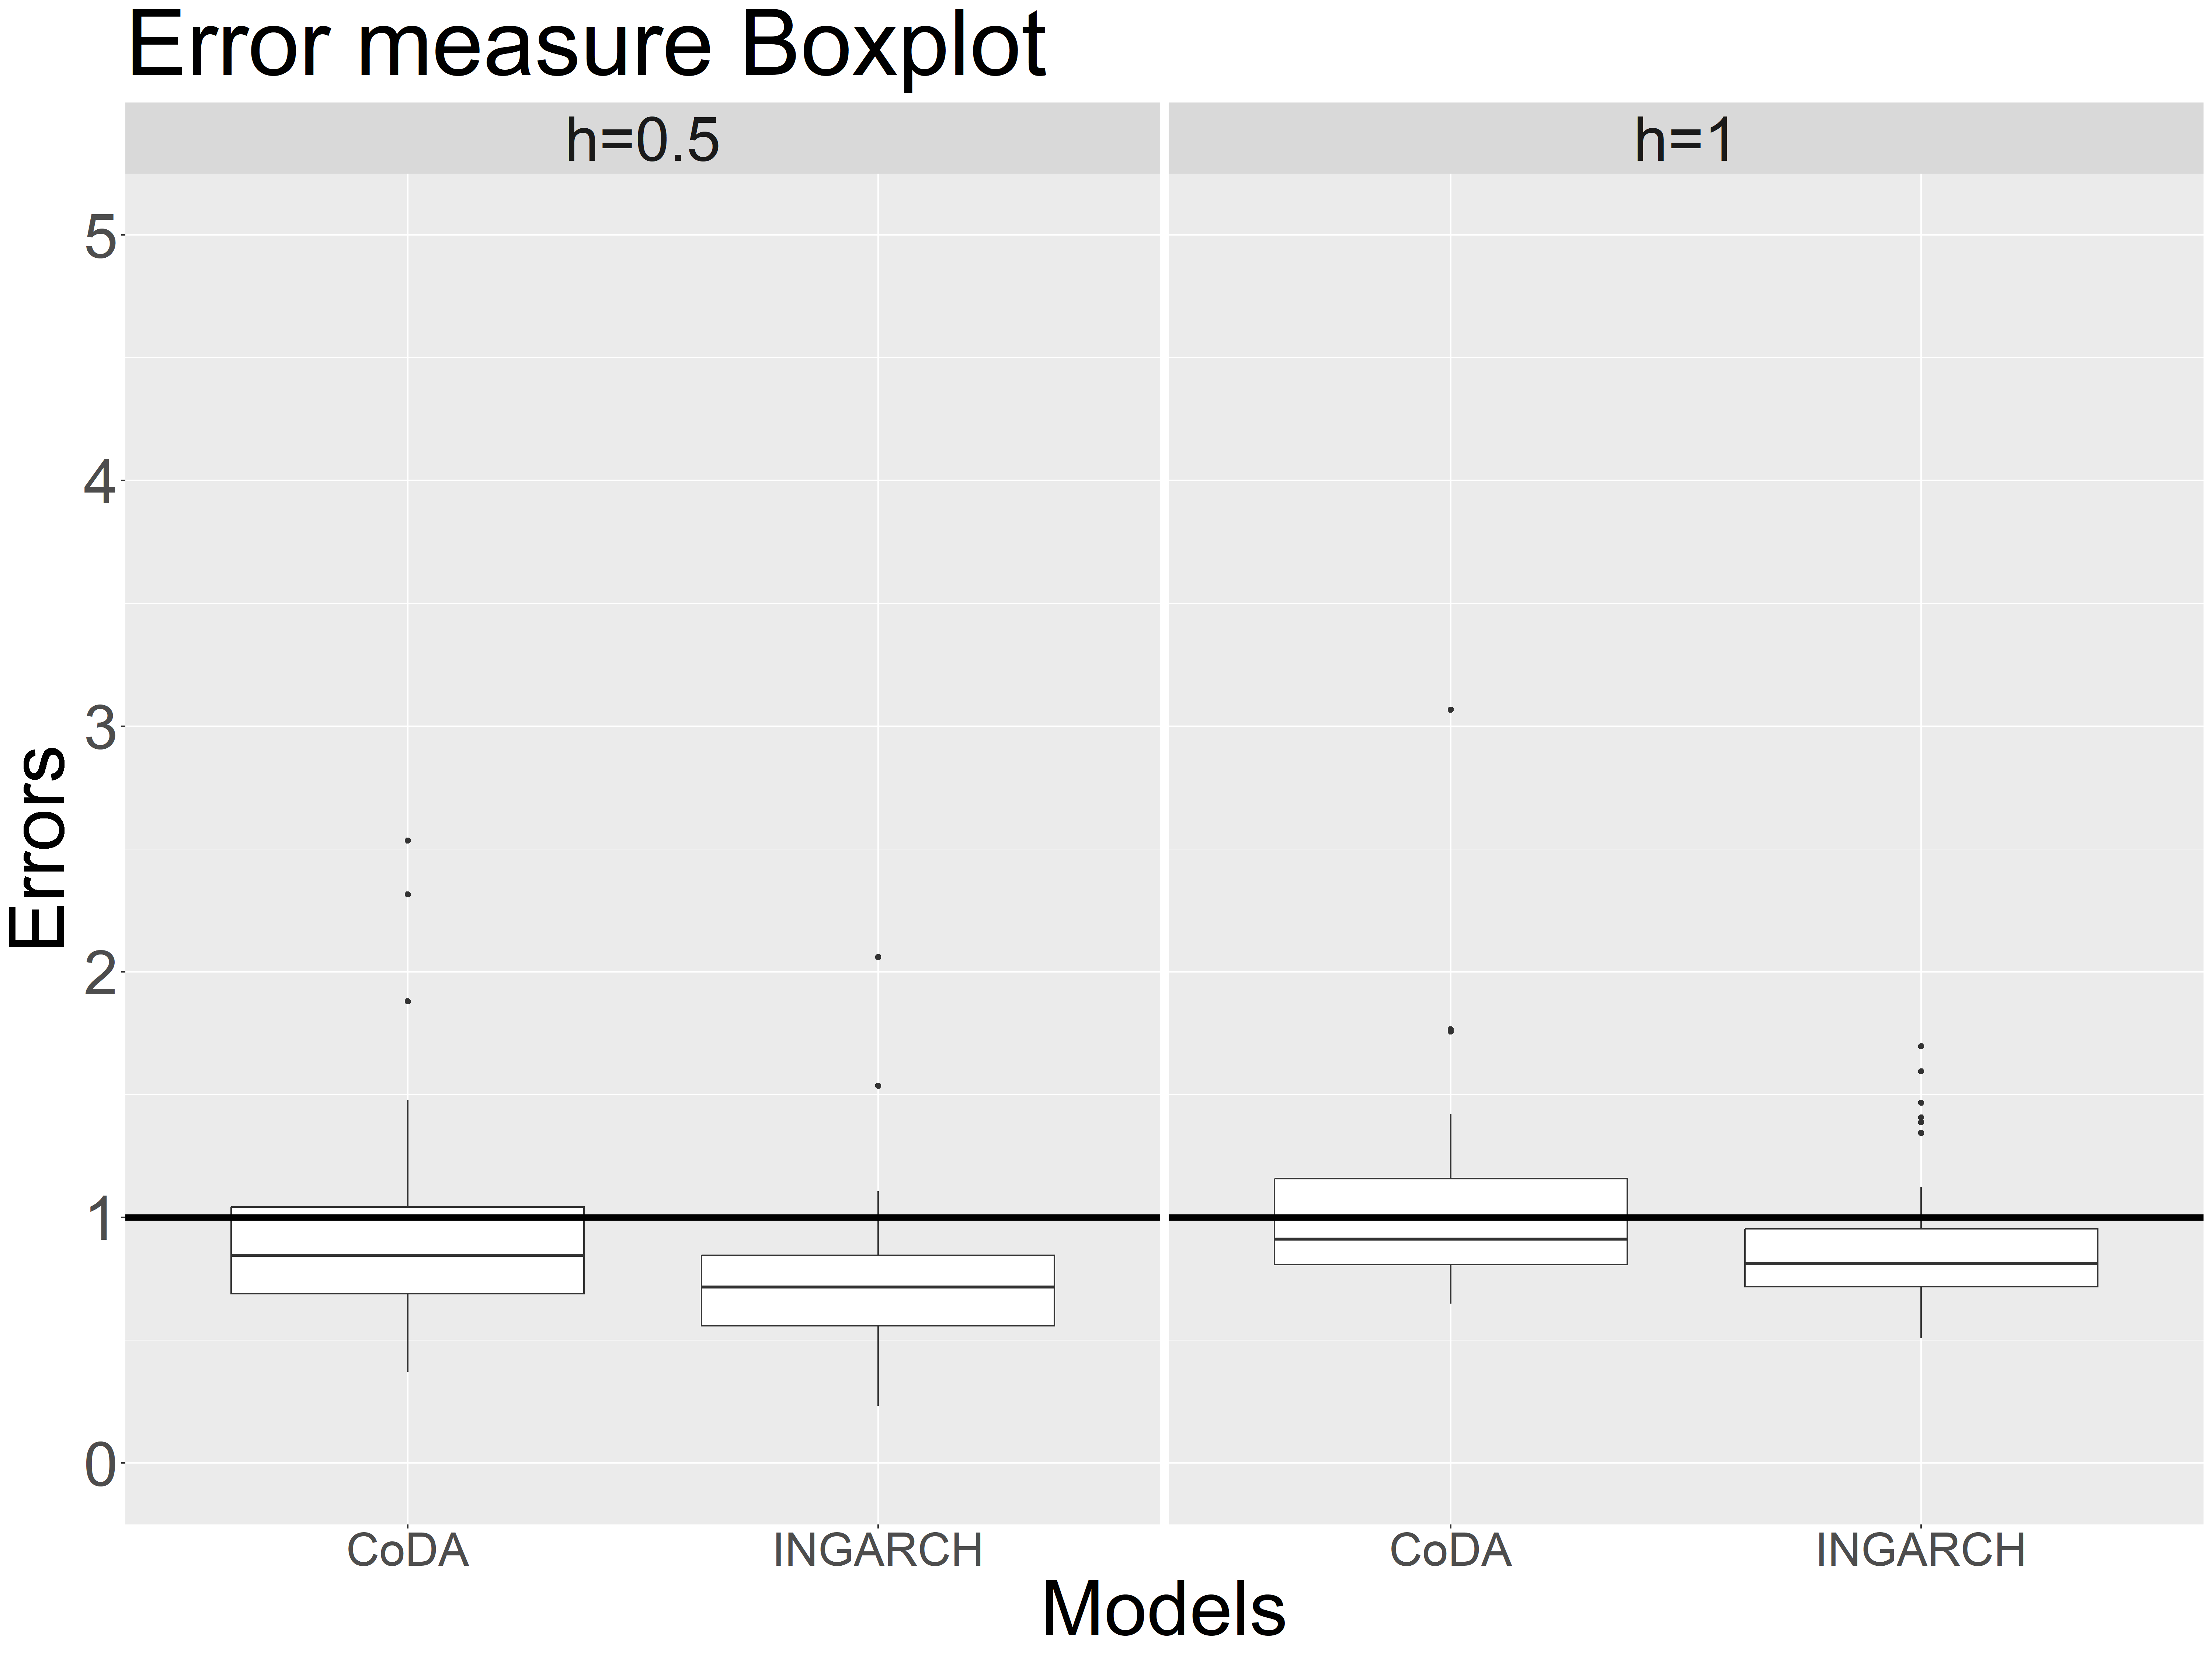
\includegraphics[width=\textwidth]{ErrorMeasureCombined_Box_all__Variation_history.png}
\caption{Boxplot for different history lengths}
\label{fig:History Box}
\end{subfigure}
\hfill
\begin{subfigure}[b]{0.45\textwidth}
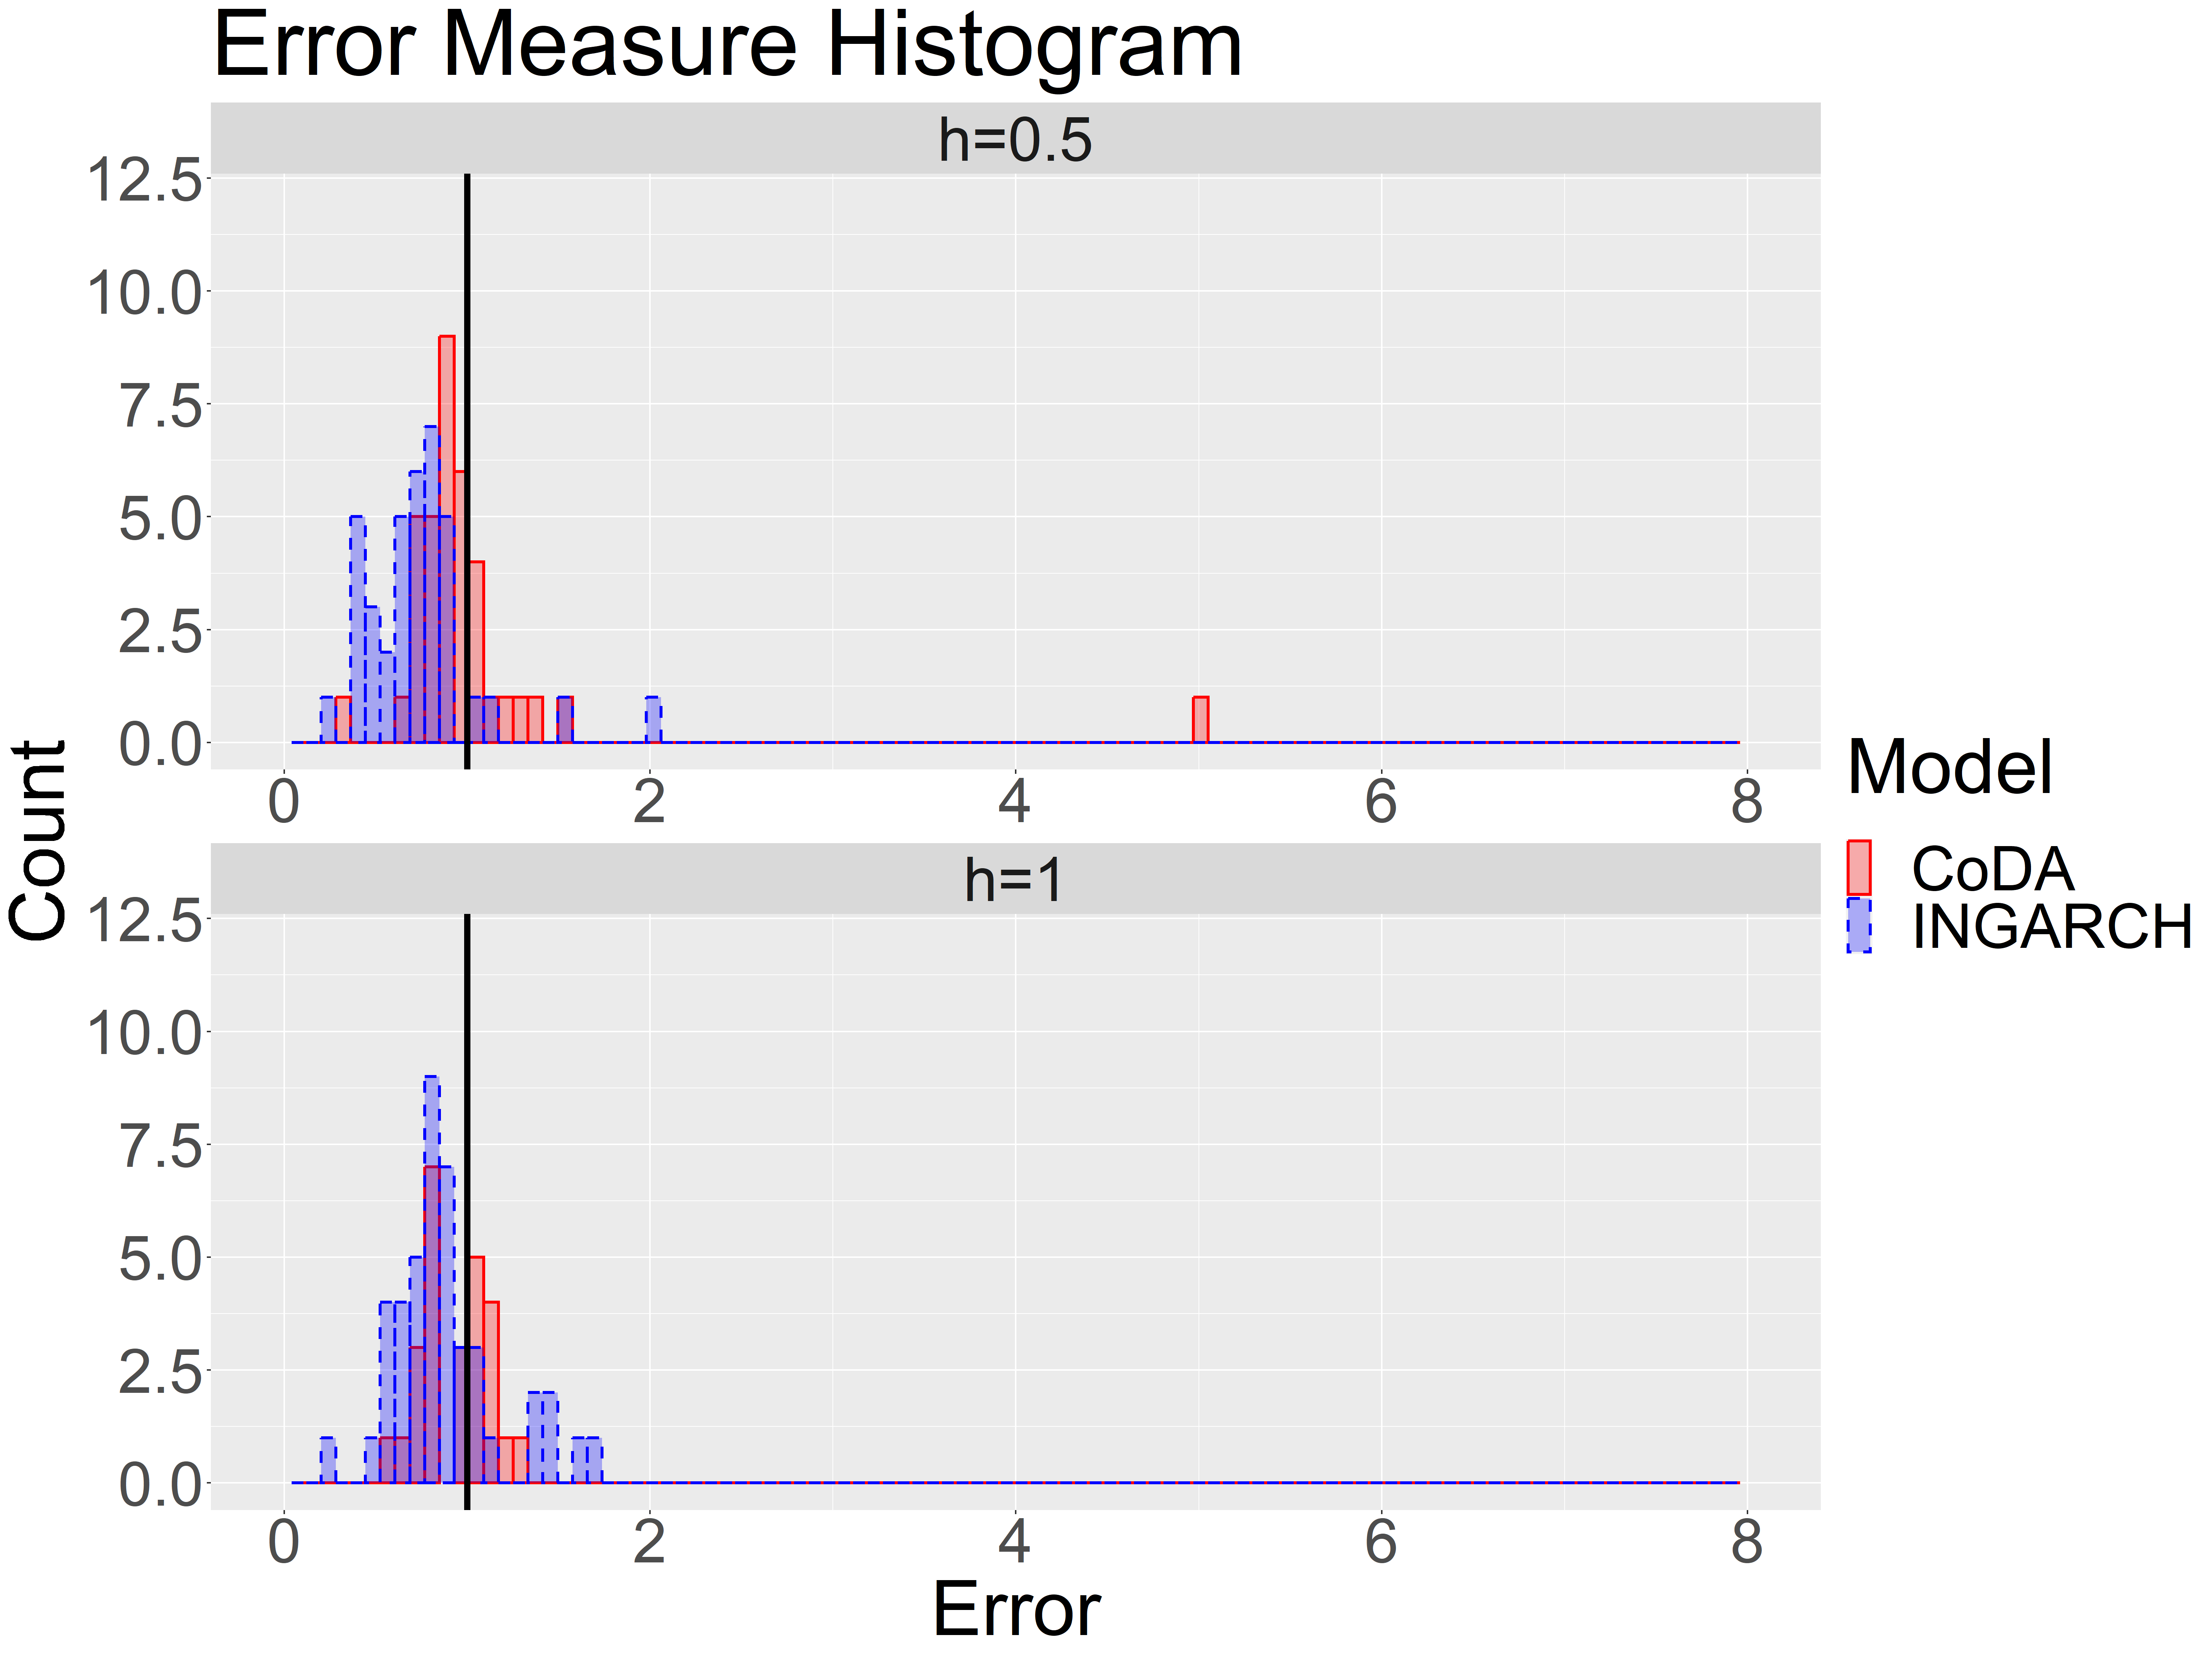
\includegraphics[width=\textwidth]{ErrorMeasureCombined_Histogram_all__Variation_history.png}
\caption{Histogram for different history lengths}
\label{fig:History Hist}
\end{subfigure}
\hfill
\begin{subfigure}[b]{0.8\textwidth}
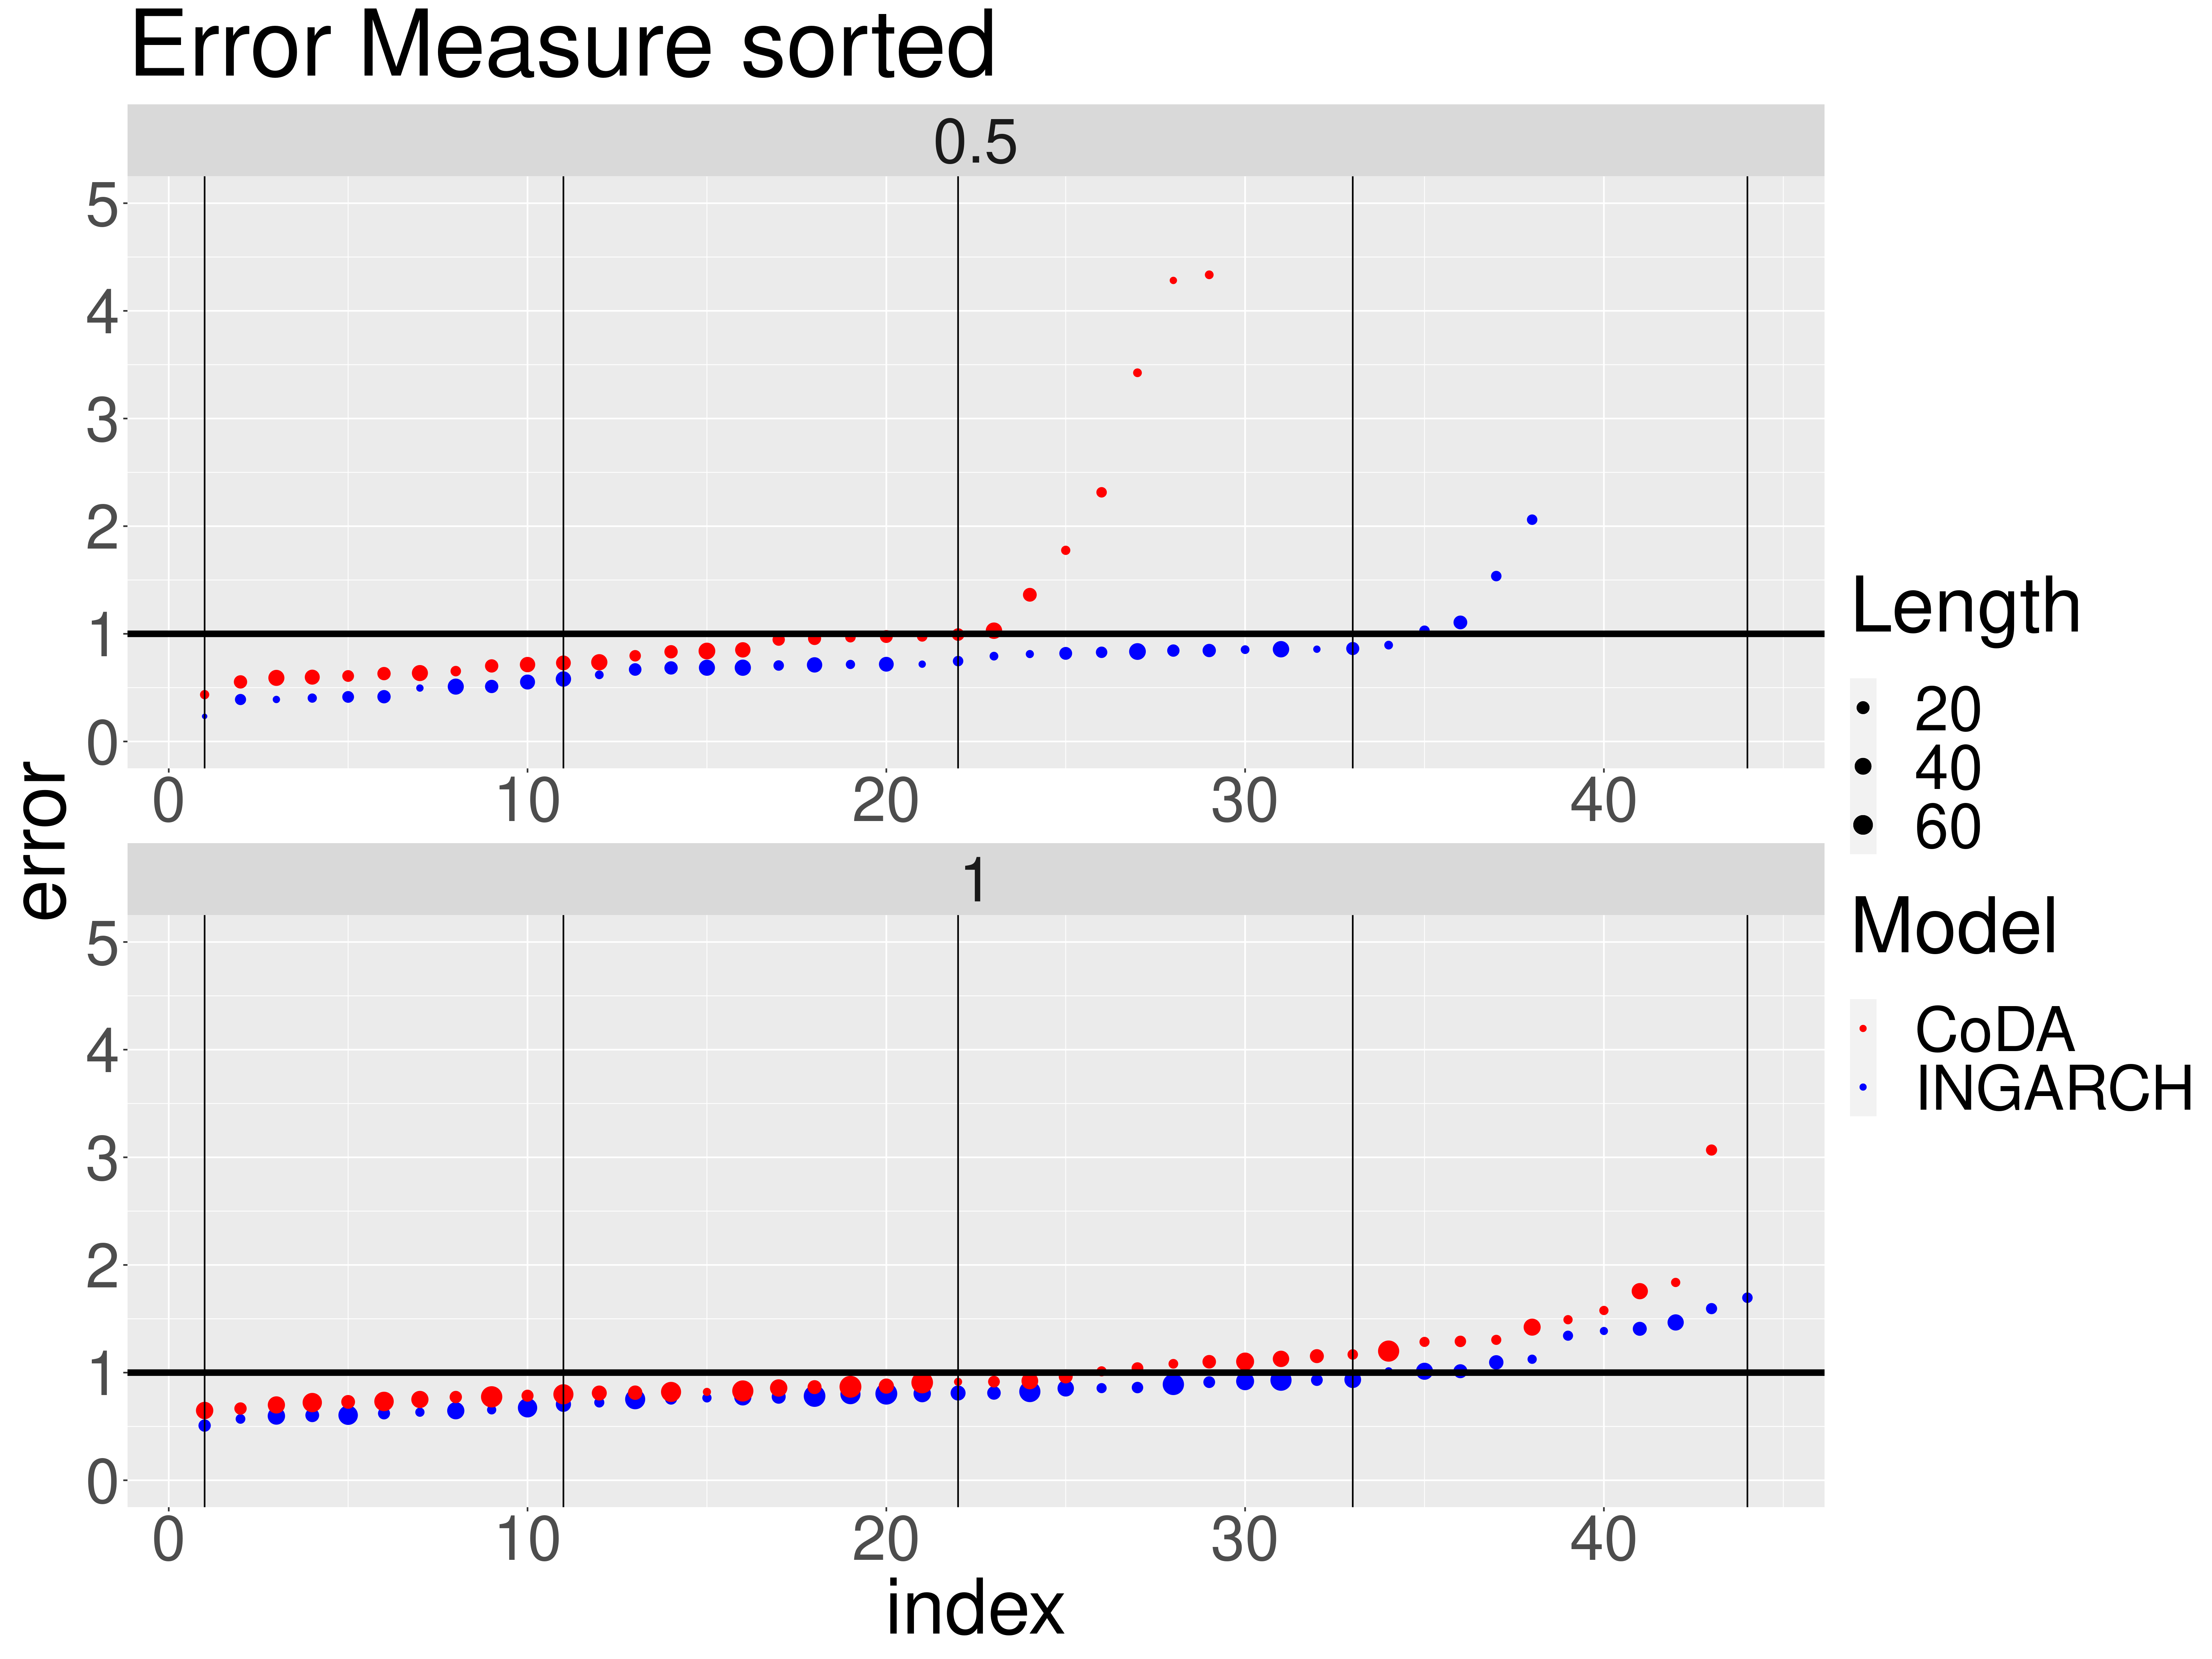
\includegraphics[width=\textwidth]{ErrorMeasureCombined_Quant_all__Variation_history.png}
\caption{Quantiles Plot for different history lengths}
\label{fig:History Quant}
\end{subfigure}
\caption{Comparison of different history lengths}
\label{fig:History Comp1}
\end{figure}

In figure \ref{fig:History Comp1} we can see that the results for CoDA vary for the different history lengths. While for a history of half of the length of the original time series, on around 75\% of the fridges the error measure is smaller than 1, this number drops to 50\% if we use the whole history. However, one can see in the quantile plot \ref{fig:History Quant} that we have 8 less values for the factor 0.5 than for 1. This means that either we have larger values than the limits of the y-axis or that the method was unable to compute any result at all. 

For INGARCH, the results are very similar. For a factor of 1 we get slightly higher values for the error measure as seen in \ref{fig:History Box}. But again in \ref{fig:History Quant} we see that we have less values for the shorter history. So again they are either too large to be shown, or there do not exist any values at all. 

\subsubsection{Frame}
\label{sec:Frame}

Next, we vary the initial frame length $w_f$. We choose to extend the frame with each new data point. In addition, we take the frame as a fraction of the history used. For example, the value $w_f=0.3$ means that 30\% of the data points are chosen for the first estimation. The results are portrayed in \ref{fig:Frame Comp1}. In general, there is not much difference between the different frames. INGARCH seems to perform better for all three values. In figure \ref{fig:Frame Quant} we can see that for CoDA some time series yielded very high errors or couldn't calculate at all. 
\begin{figure}[htb!]
\centering
\begin{subfigure}[b]{0.45\textwidth}
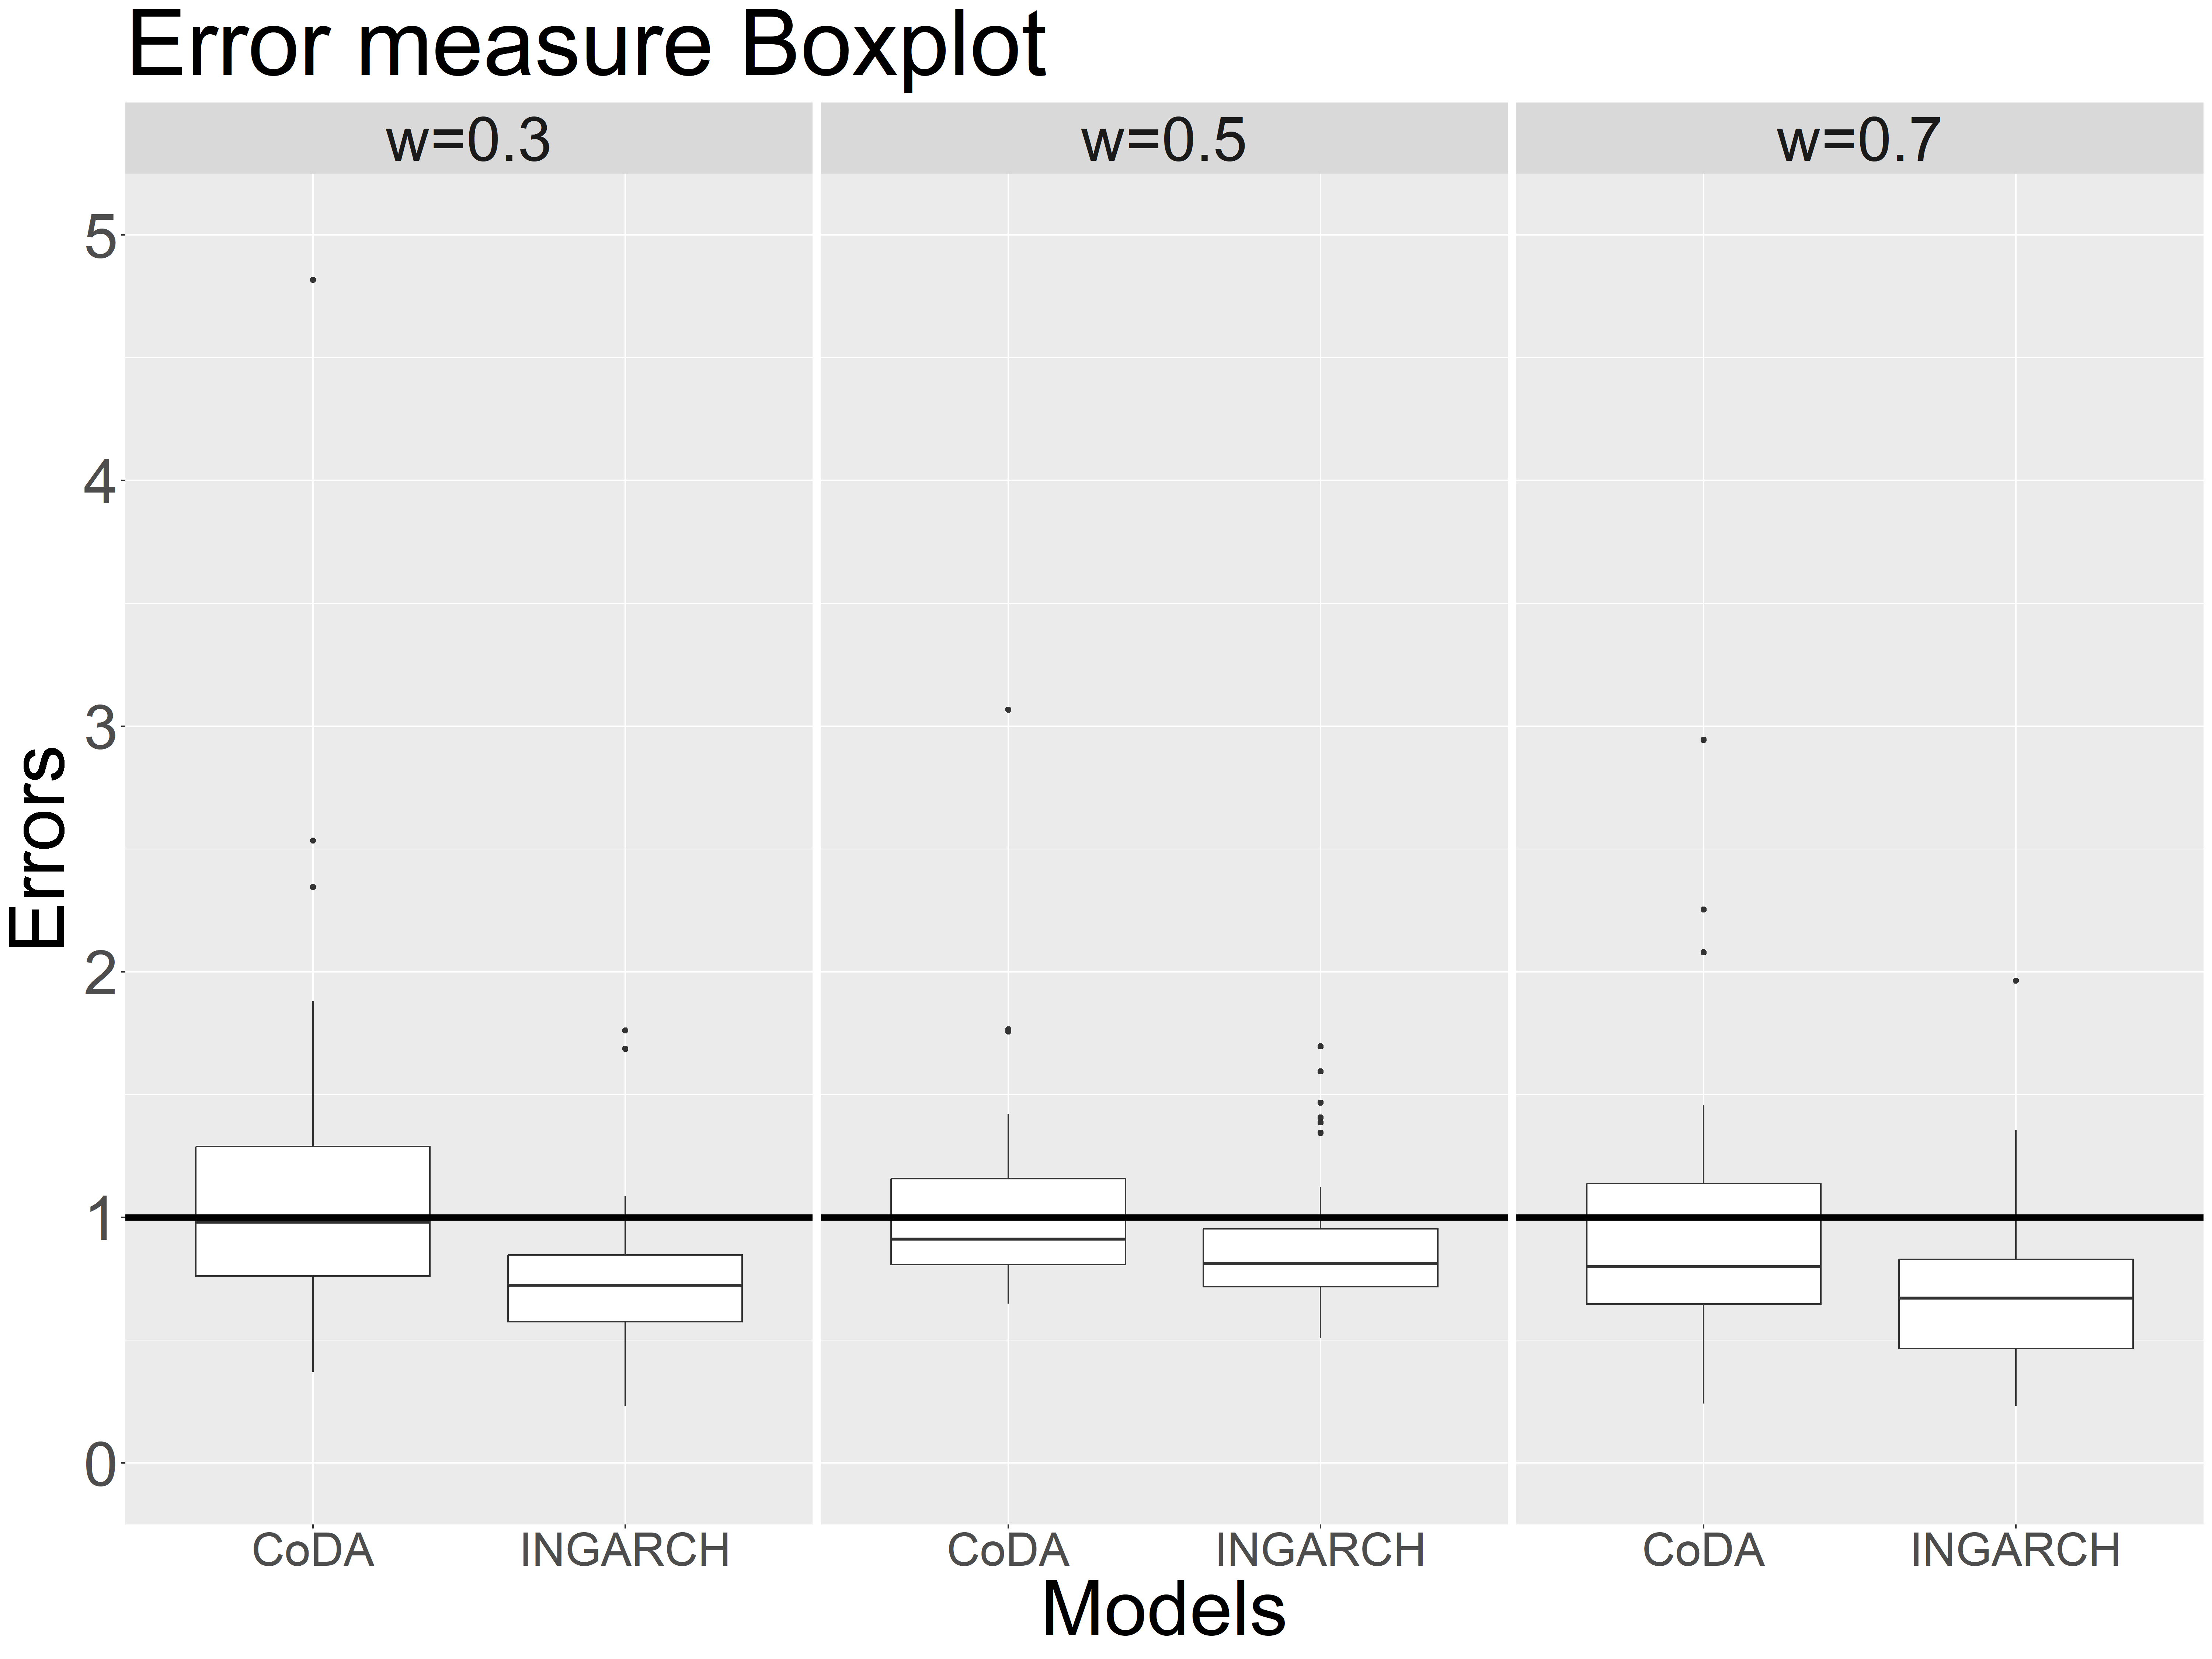
\includegraphics[width=\textwidth]{ErrorMeasureCombined_Box_all__Variation_frame.png}
\caption{Boxplot for different frames}
\label{fig:Frame Box}
\end{subfigure}
\hfill
\begin{subfigure}[b]{0.45\textwidth}
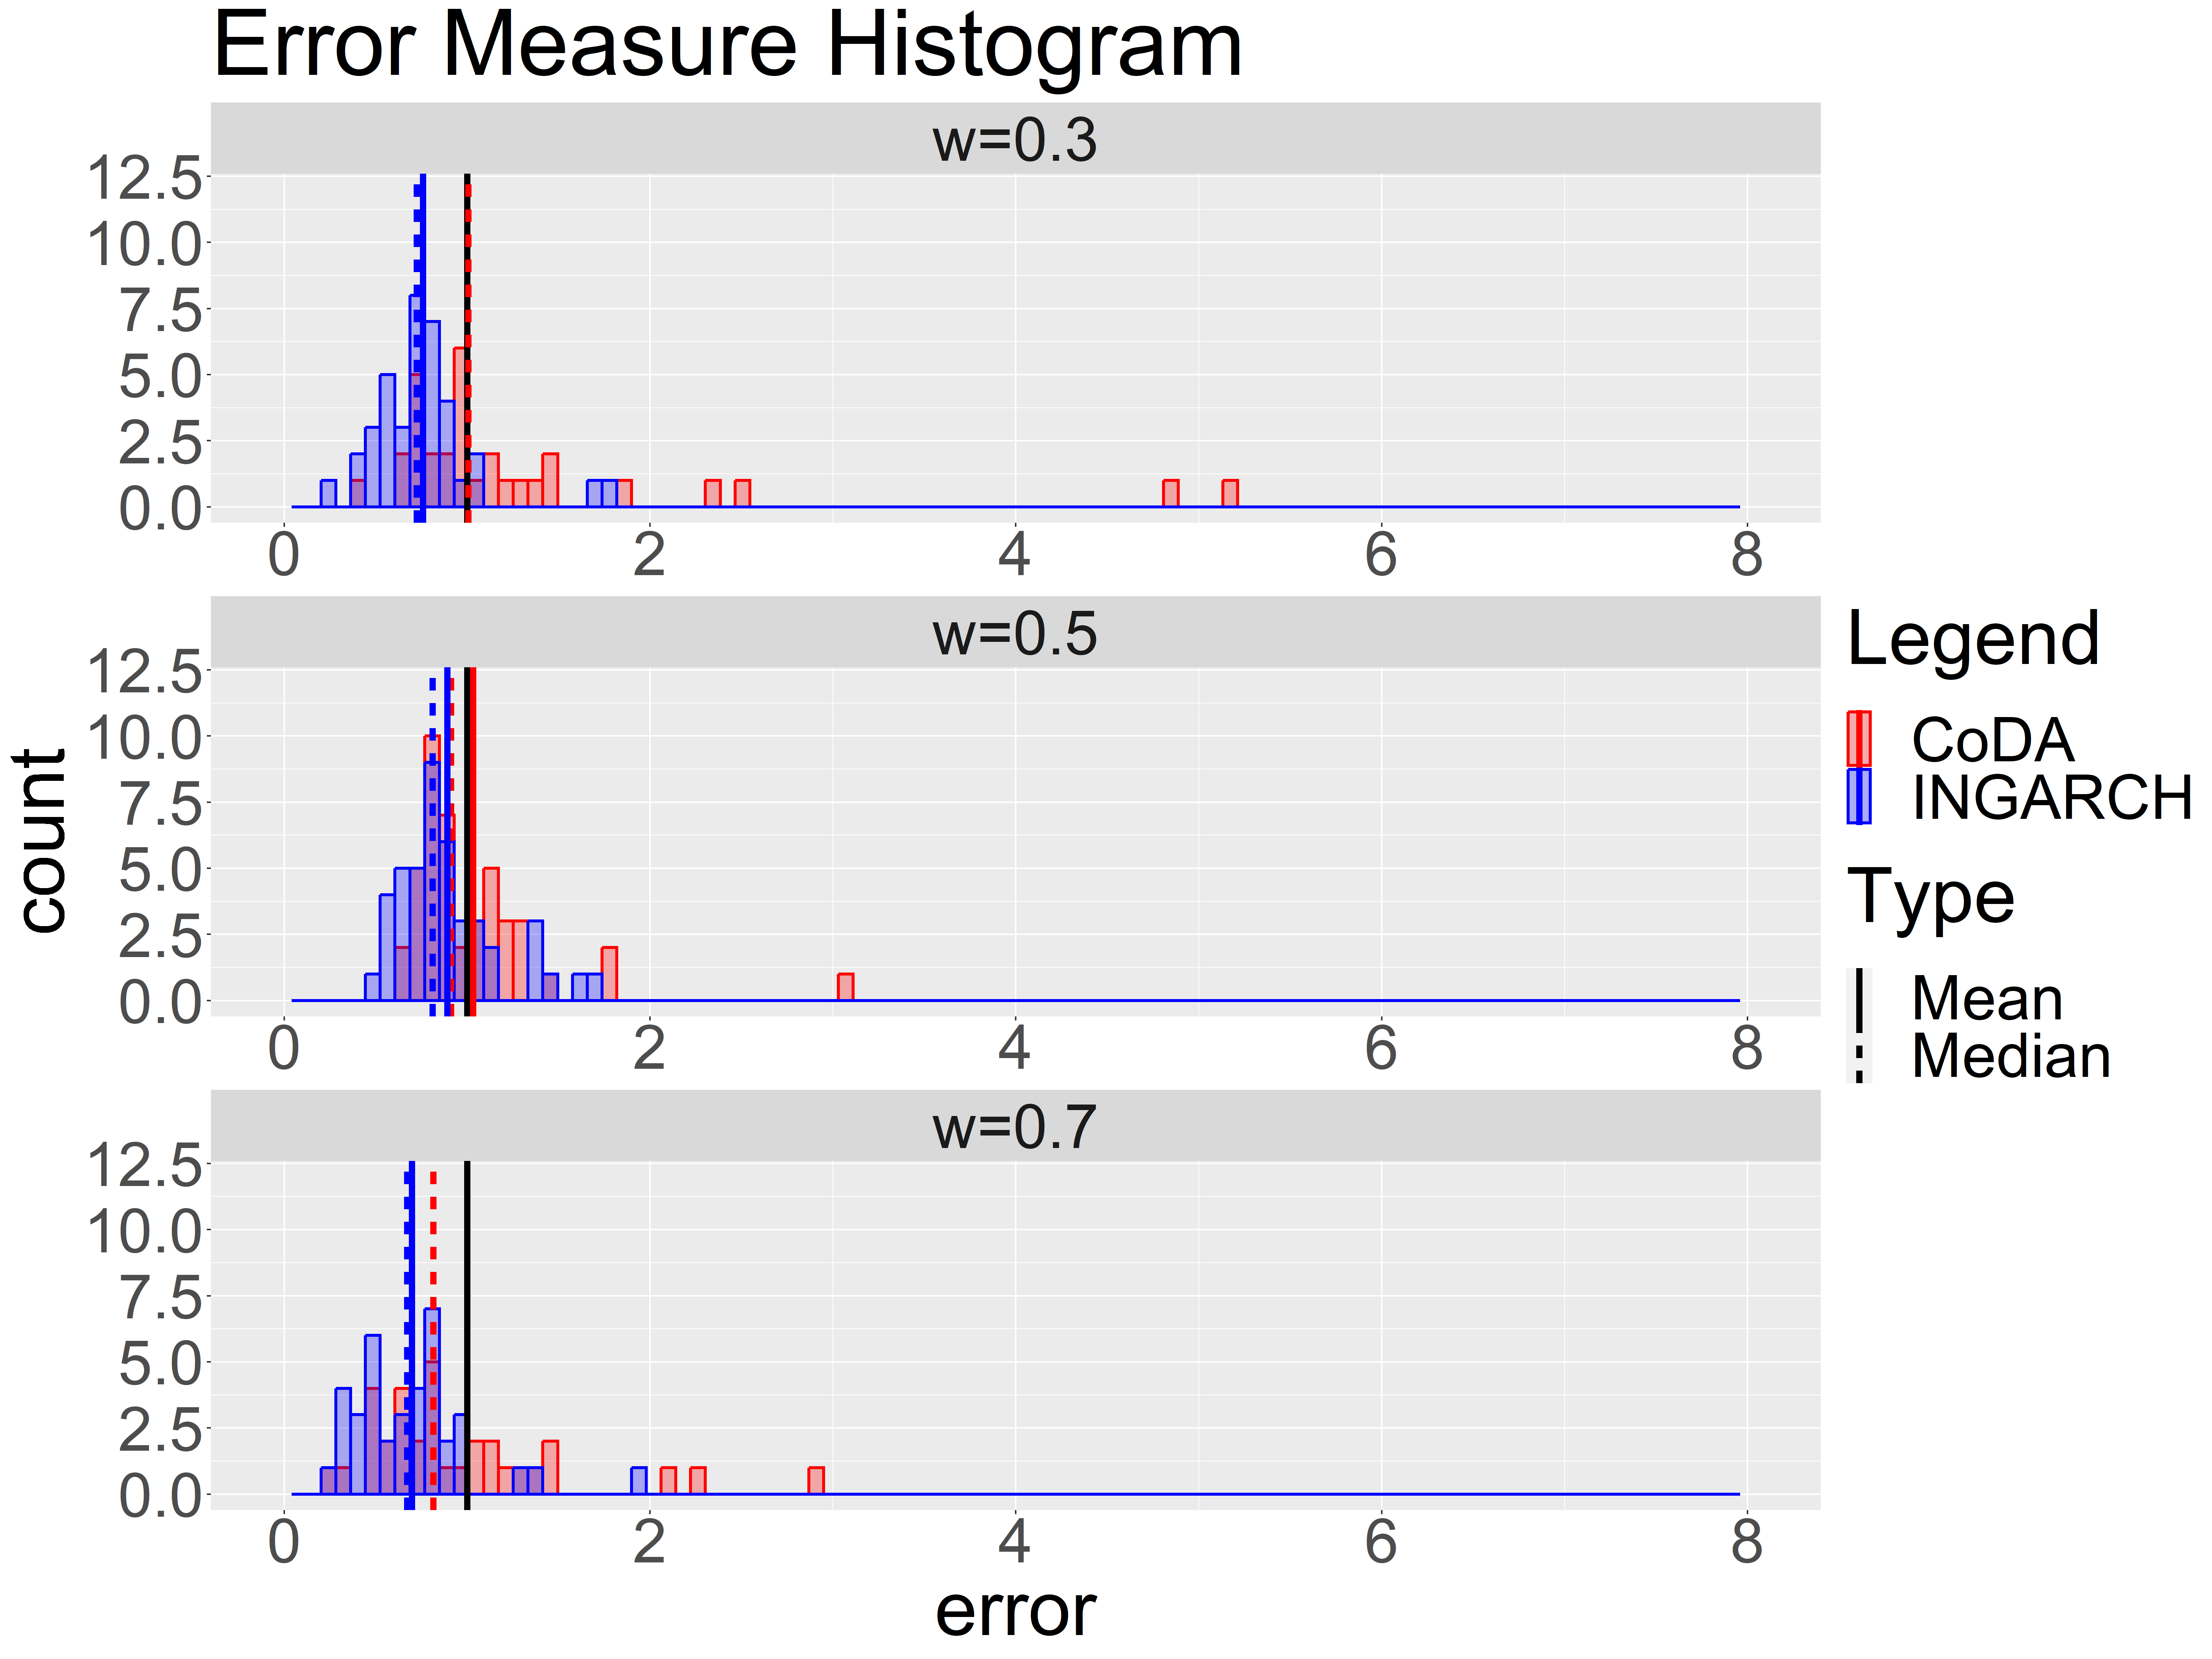
\includegraphics[width=\textwidth]{ErrorMeasureCombined_Histogram_all__Variation_frame.png}
\caption{Histogram for different frames}
\label{fig:Frame Hist}
\end{subfigure}
\hfill
\begin{subfigure}[b]{0.8\textwidth}
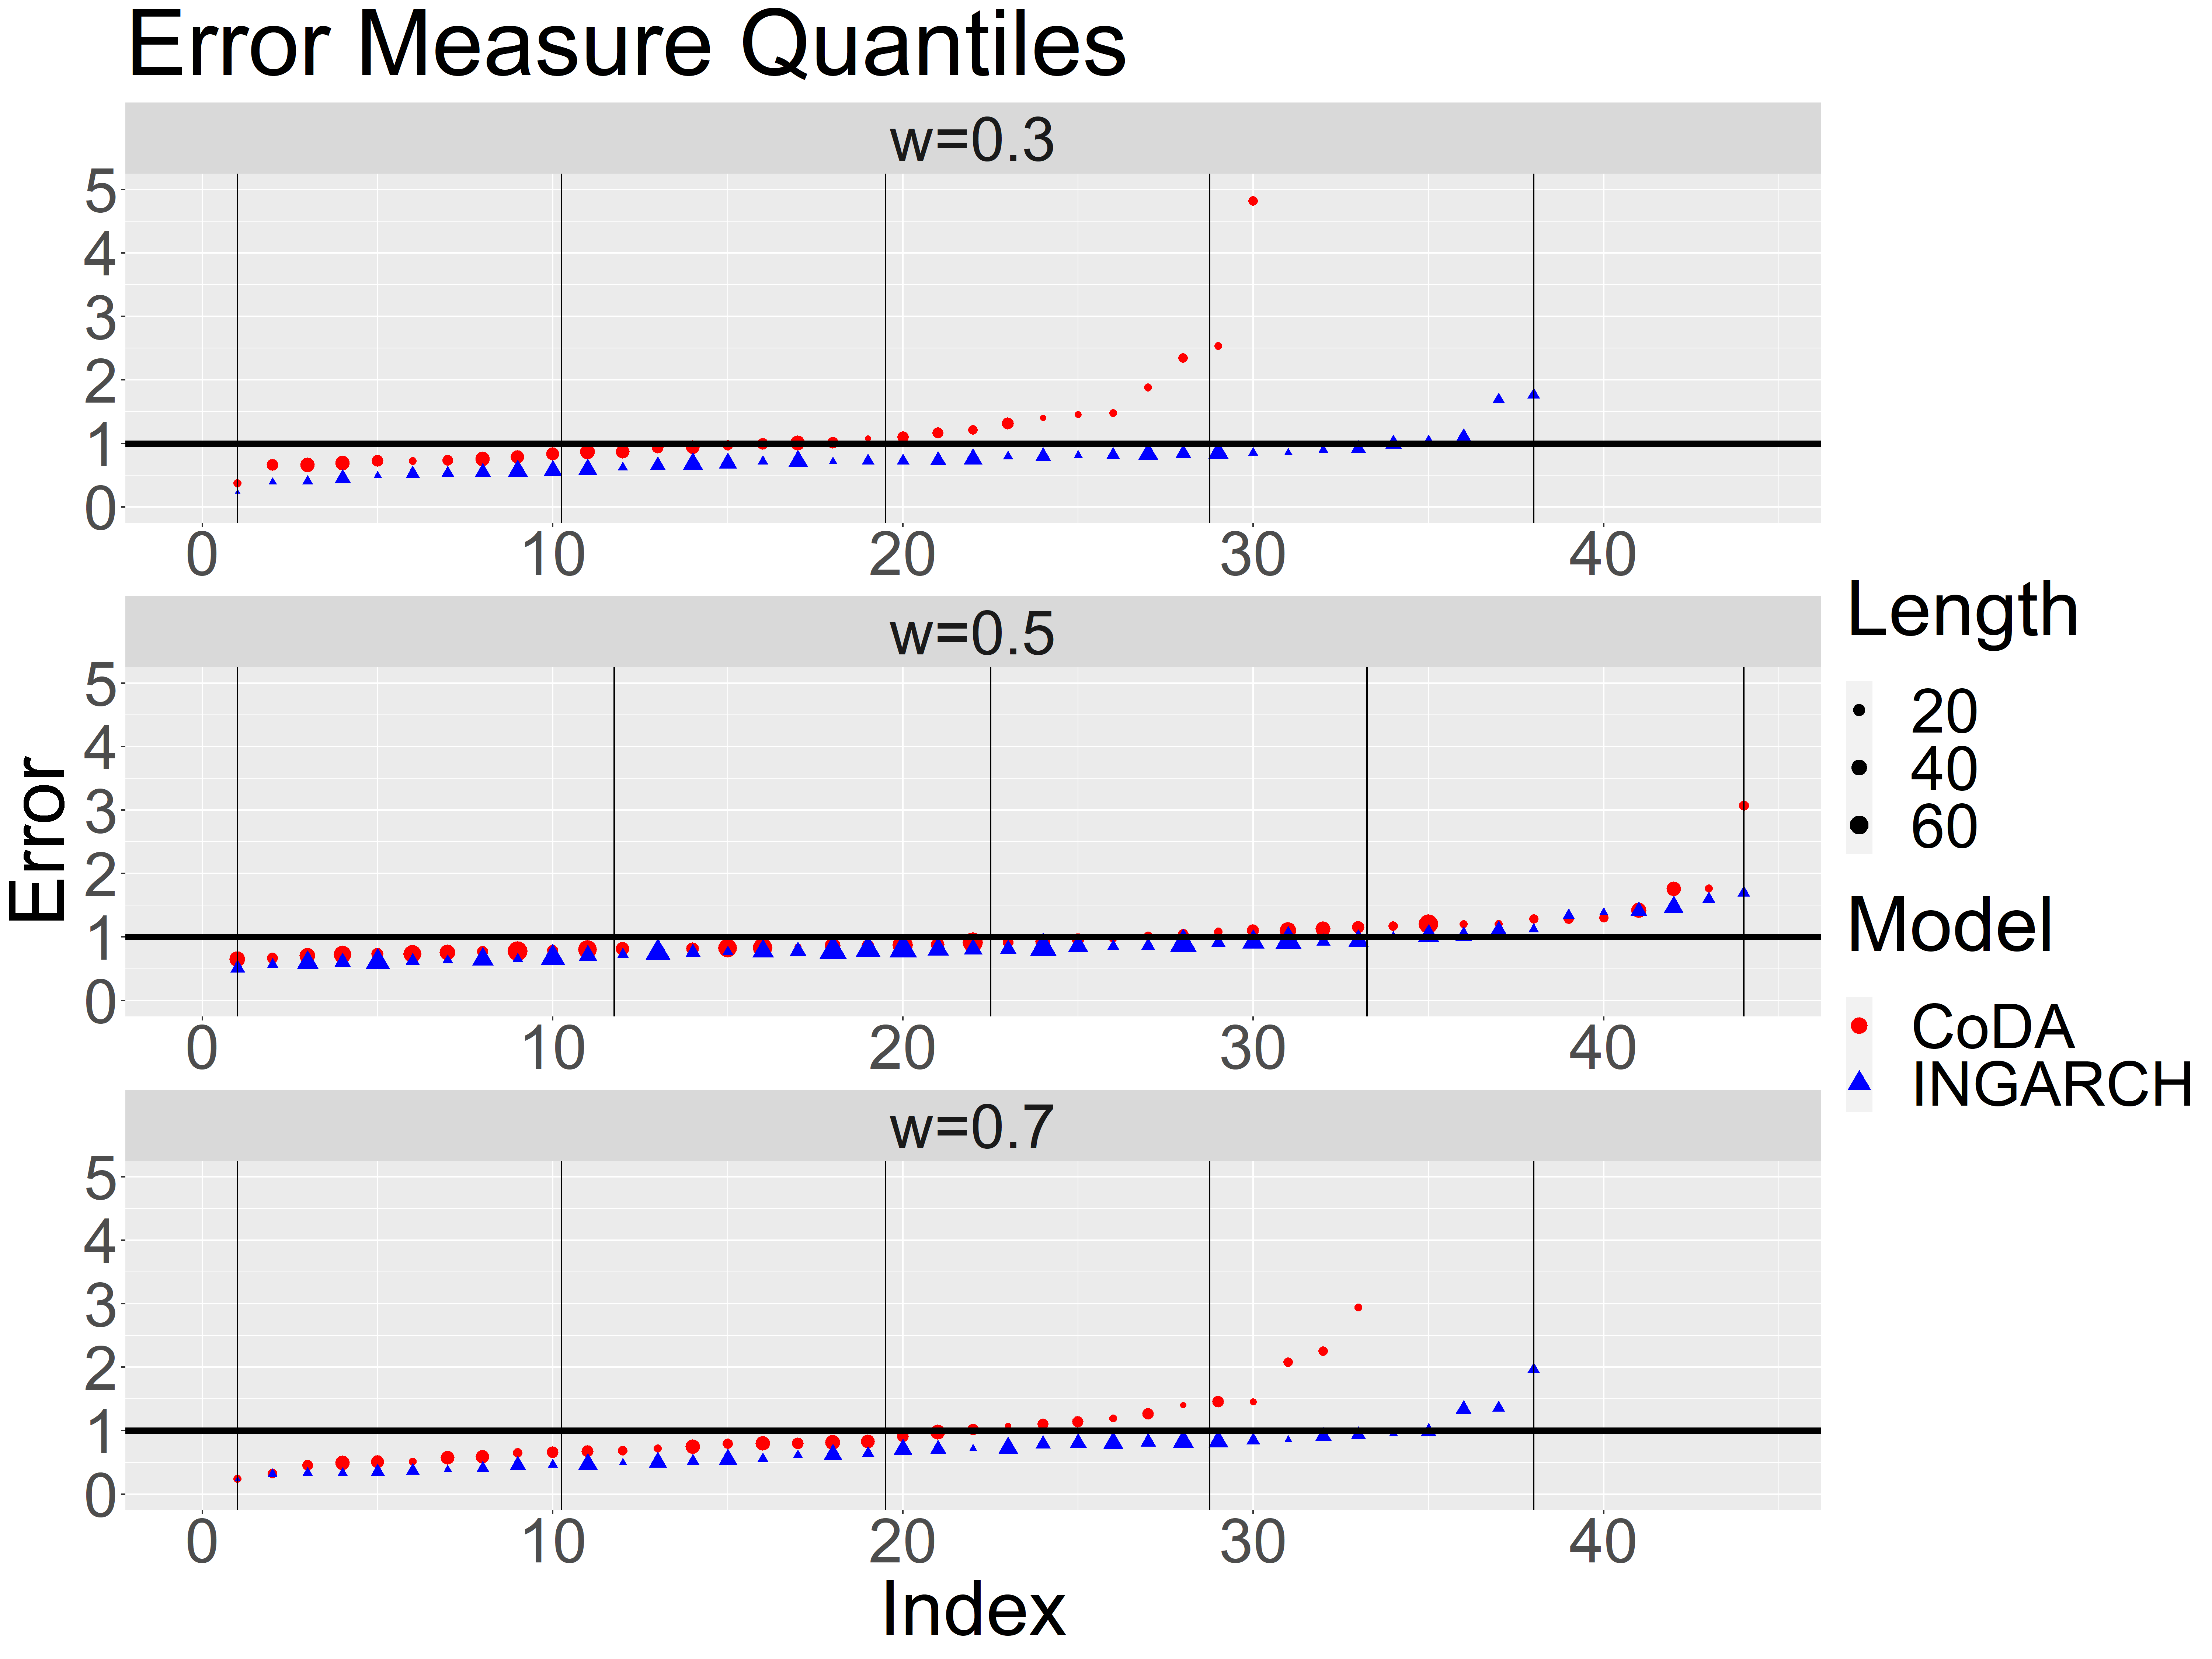
\includegraphics[width=\textwidth]{ErrorMeasureCombined_Quant_all__Variation_frame.png}
\caption{Quantiles for different frames}
\label{fig:Frame Quant}
\end{subfigure}
\caption{Comparison of different frames}
\label{fig:Frame Comp1}
\end{figure}



\subsubsection{Window Shape}
\label{sec:Window Shape}

We also vary the shape of the window. As explained in \ref{sec: Model Specification} we either use a fixed amount of points and add and remove points as time goes on, or we continuously add points to the window. The results are in figures \ref{fig:window methods Comp1}. We can see that there are no big differences between the methods. For CoDA it seems that the fixed methods has some struggles for certain fridges \ref{fig:window methods Hist}. For INGARCH there is no notable difference. 

\begin{figure}[htb!]
\centering
\begin{subfigure}[b]{0.45\textwidth}
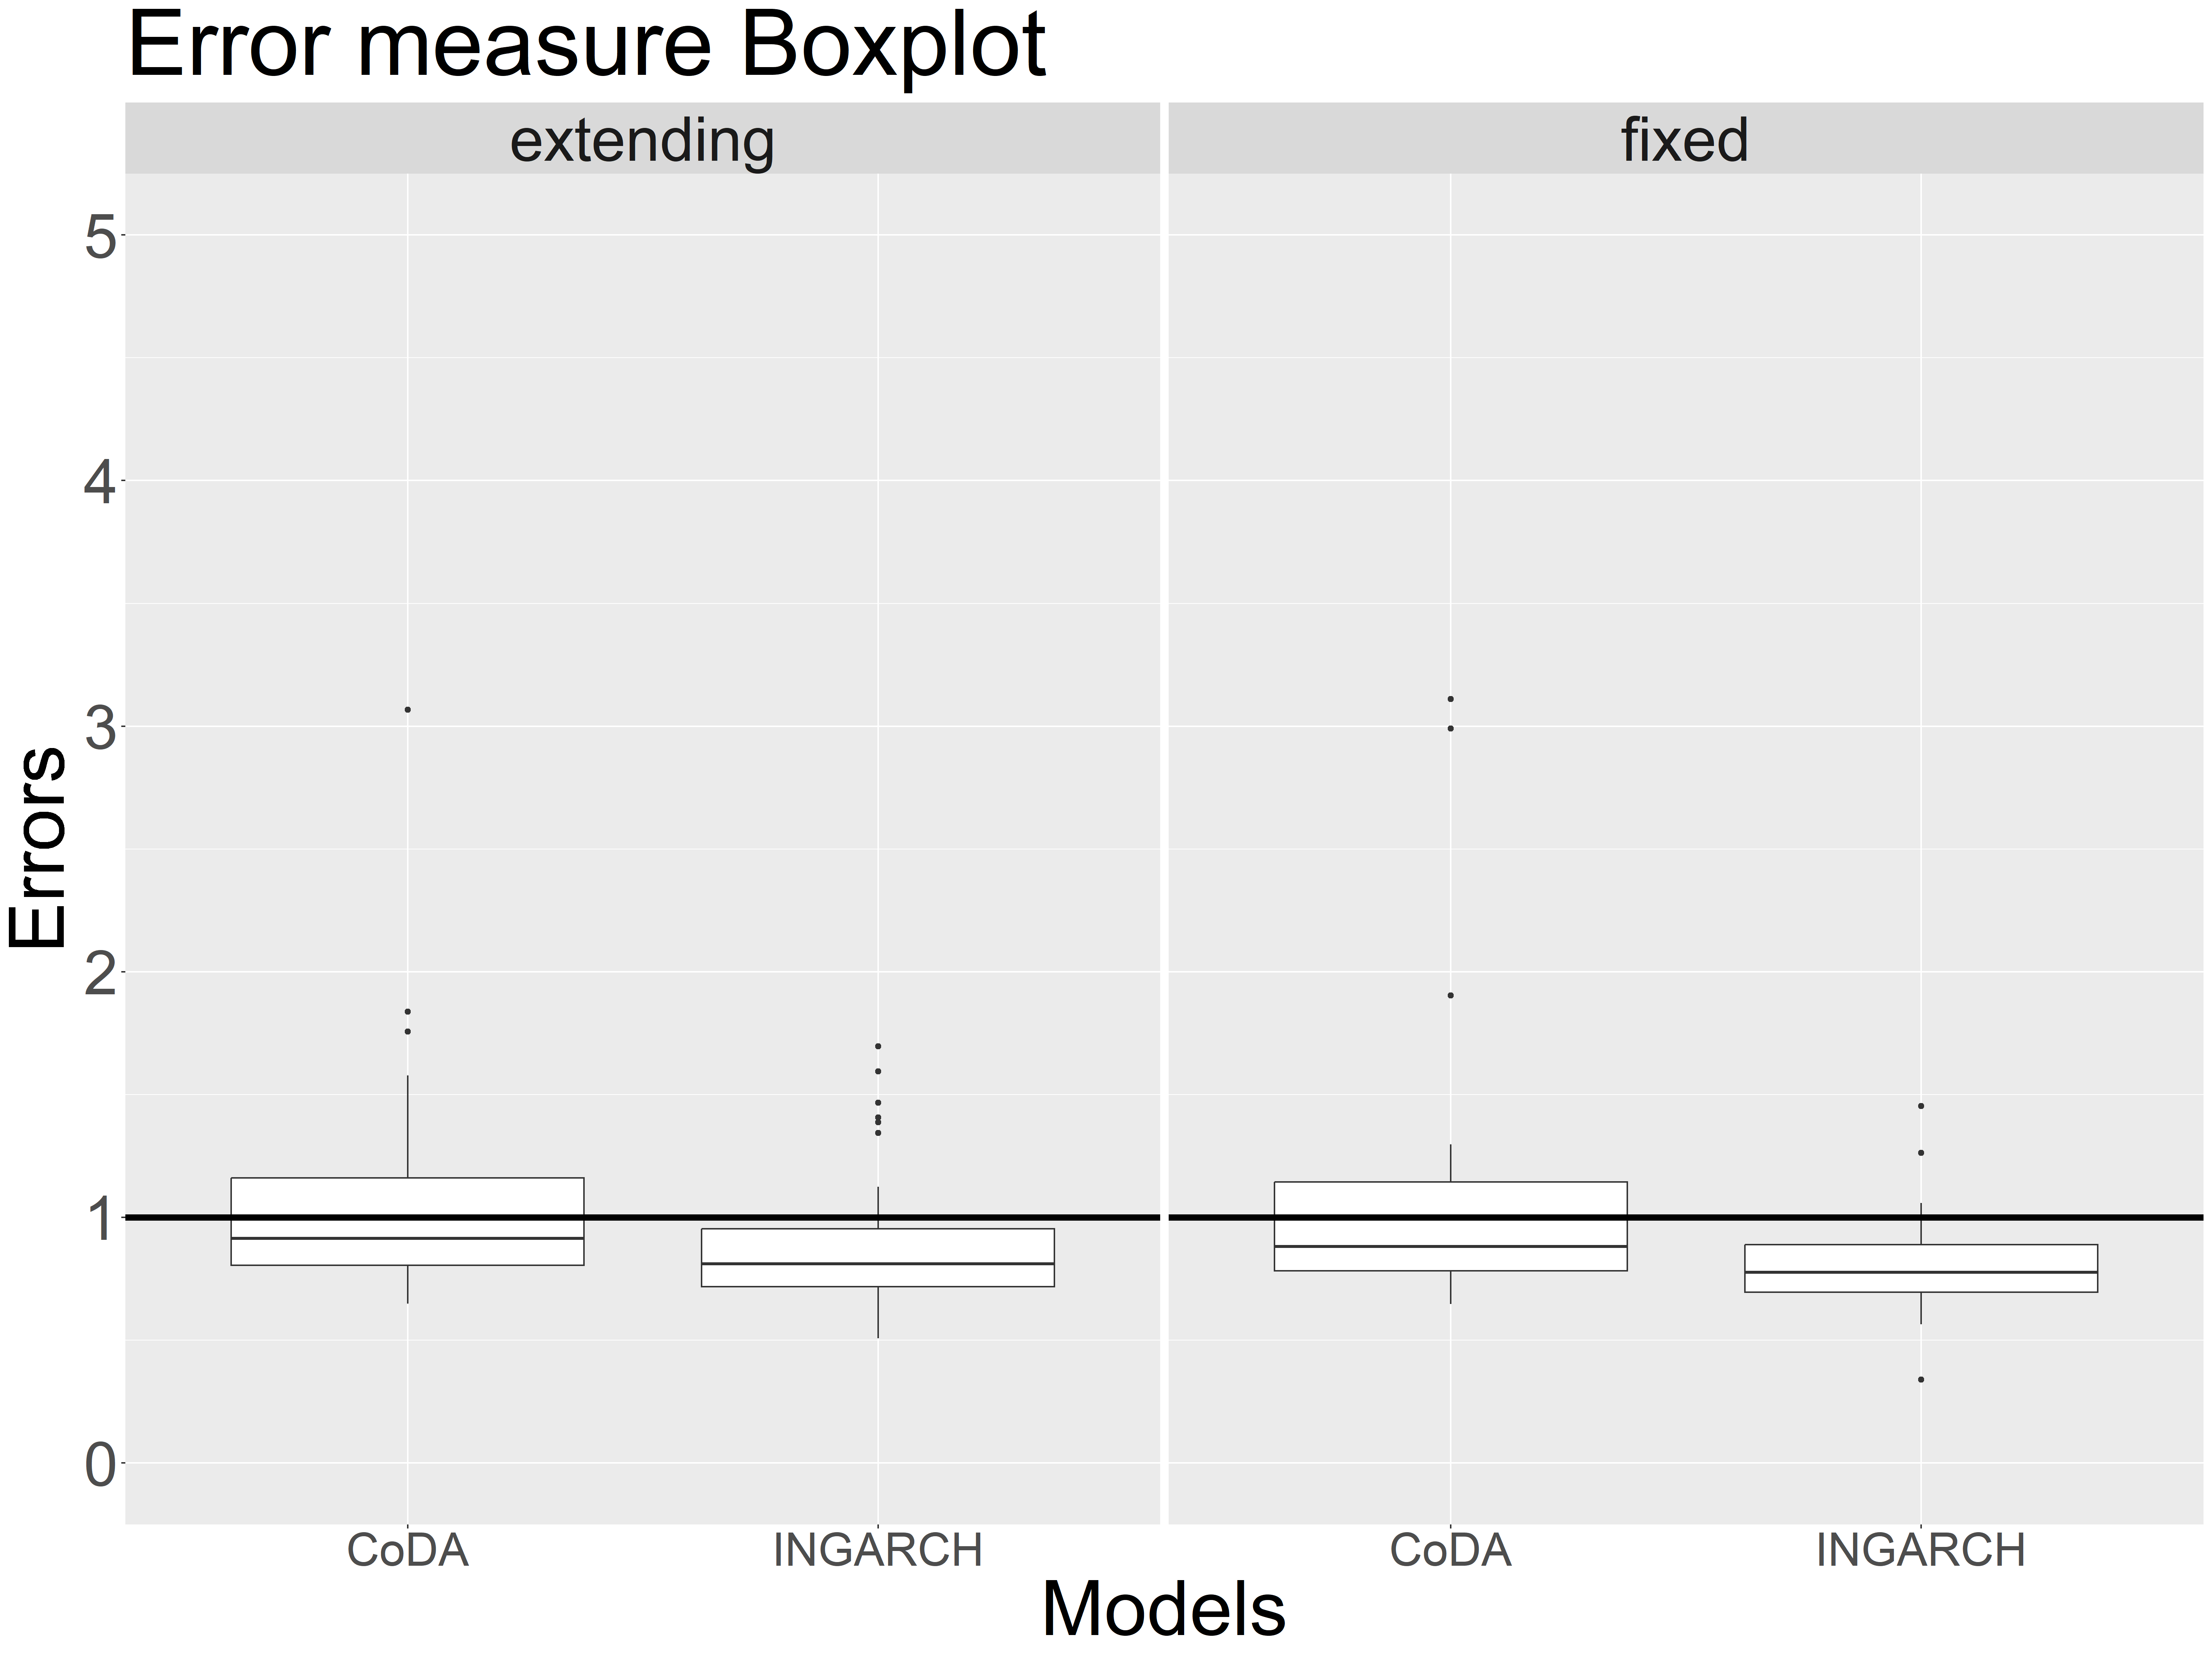
\includegraphics[width=\textwidth]{ErrorMeasureCombined_Box_all__Variation_windowMethod.png}
\caption{Boxplot for different window shapes}
\label{fig:window methods Box}
\end{subfigure}
\hfill
\begin{subfigure}[b]{0.45\textwidth}
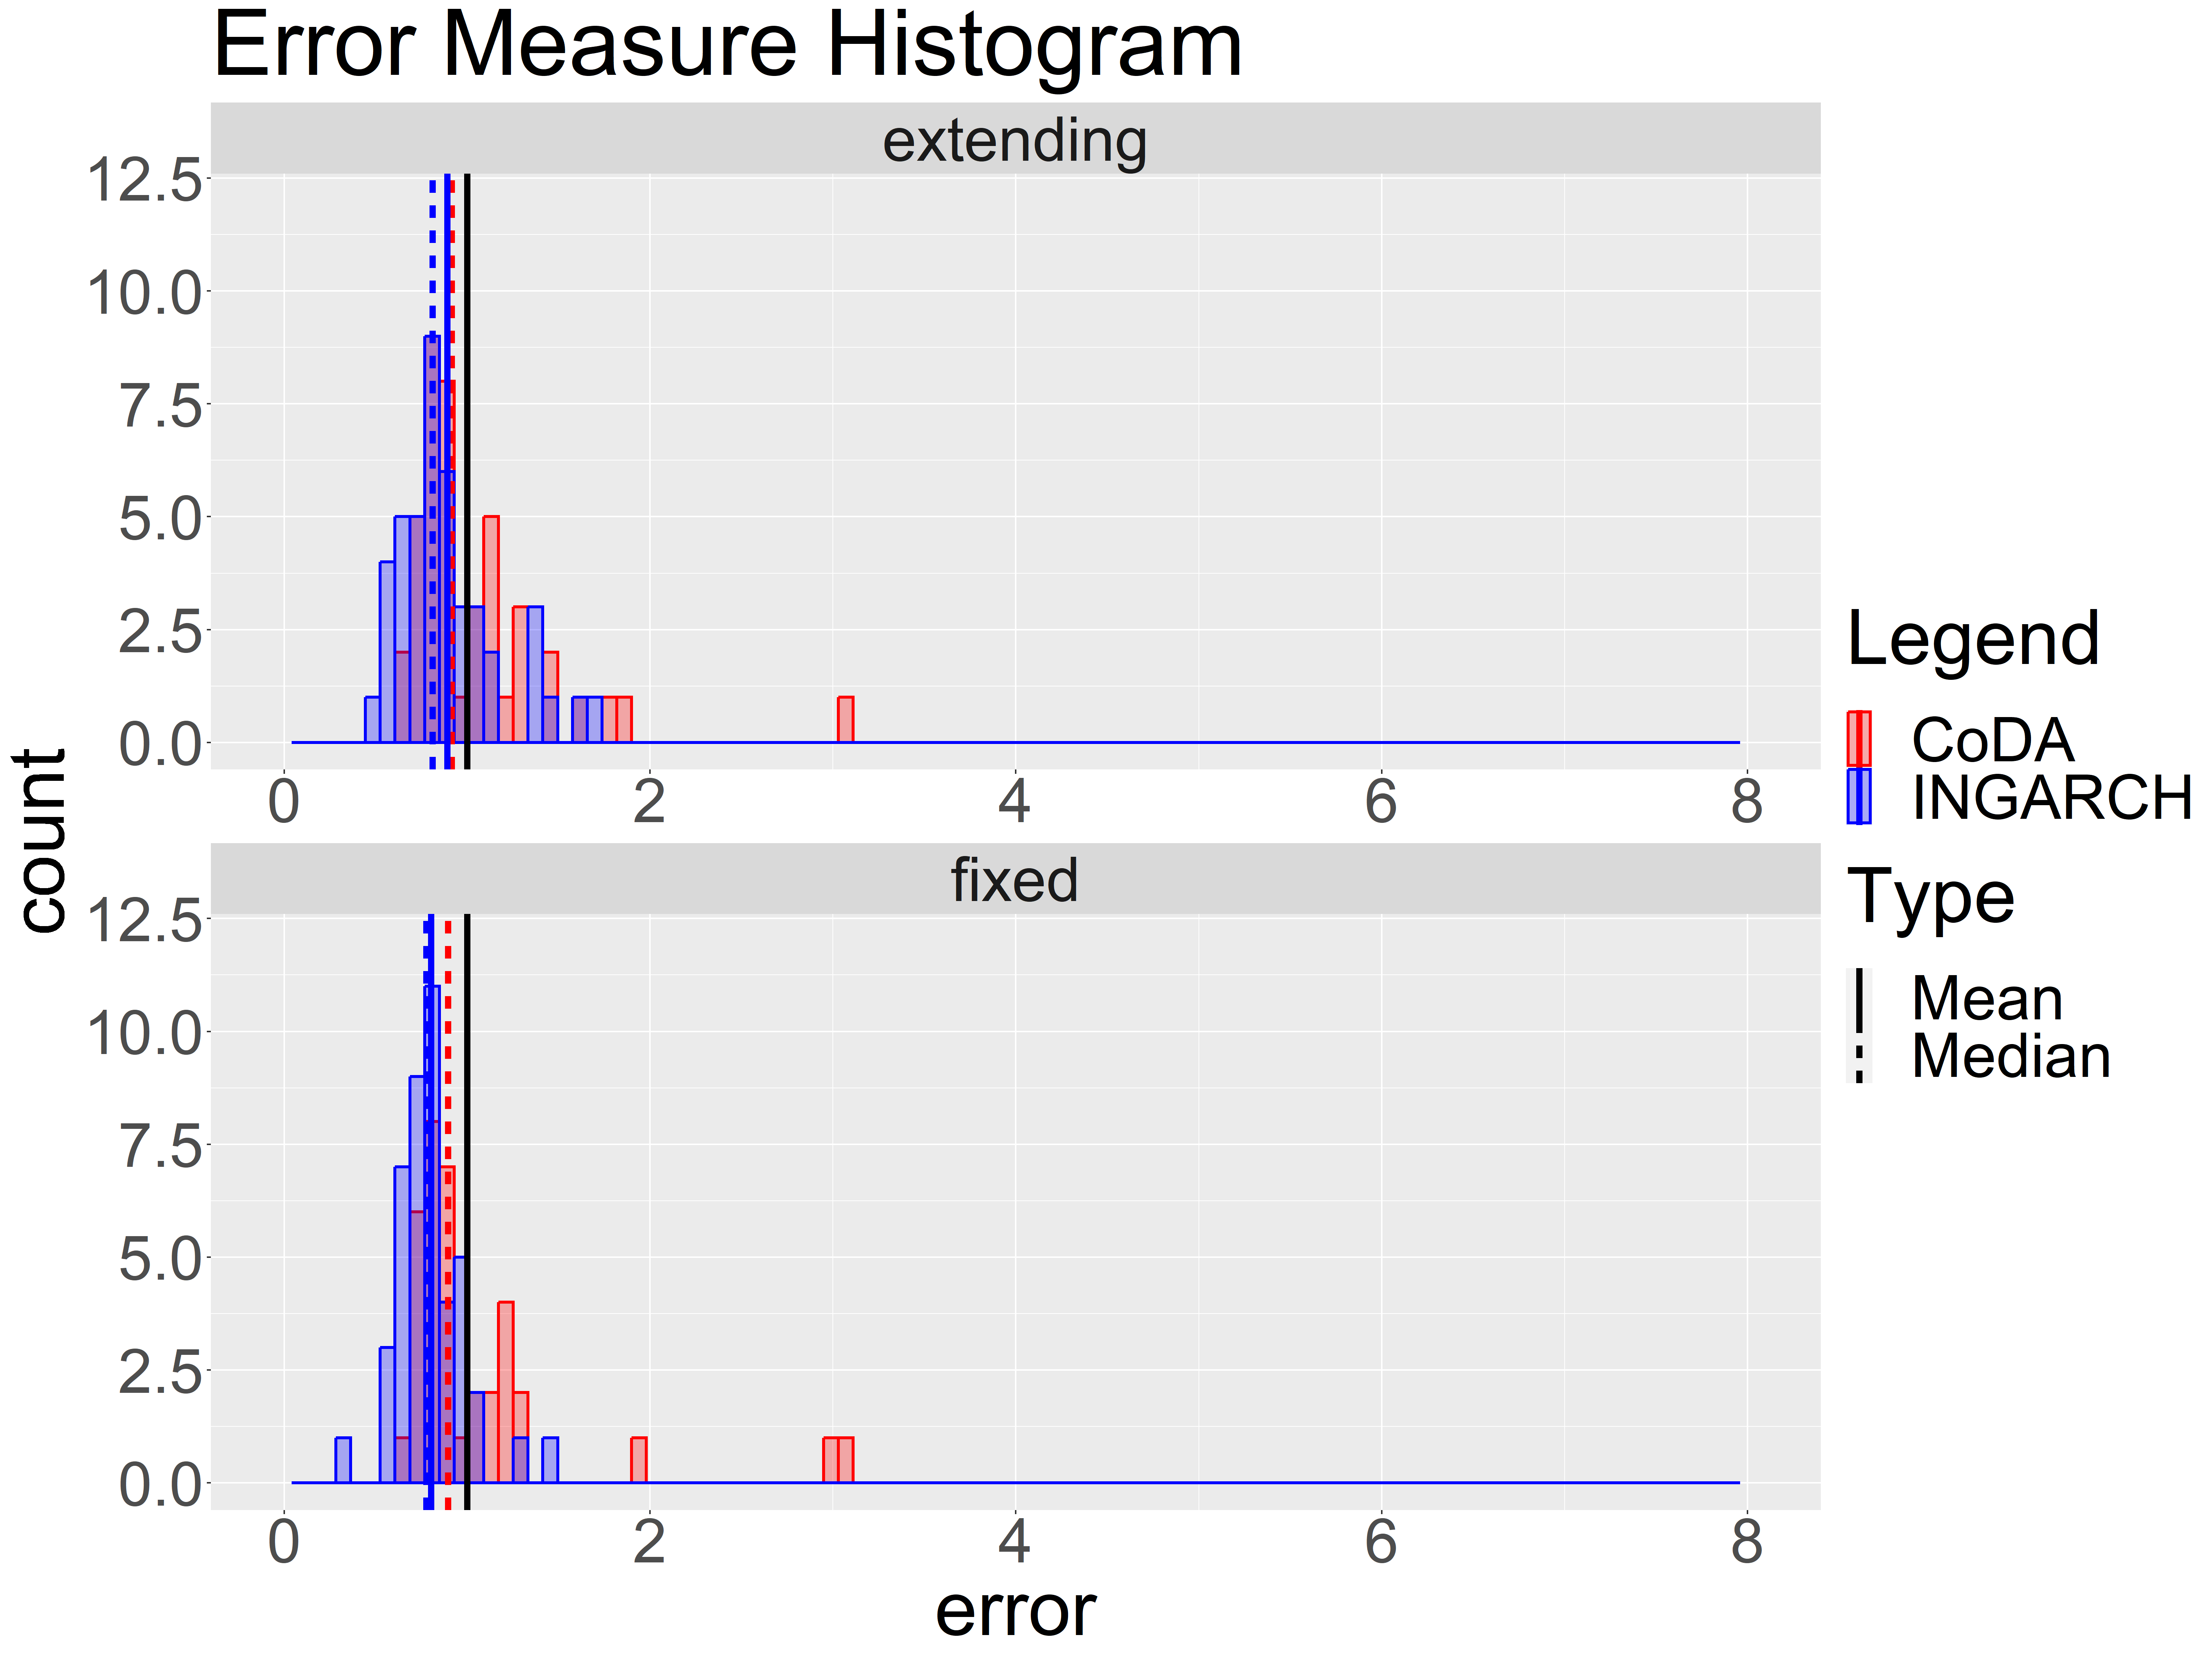
\includegraphics[width=\textwidth]{ErrorMeasureCombined_Histogram_all__Variation_windowMethod.png}
\caption{Histogram for different window shapes}
\label{fig:window methods Hist}
\end{subfigure}
\hfill
\begin{subfigure}[b]{0.8\textwidth}
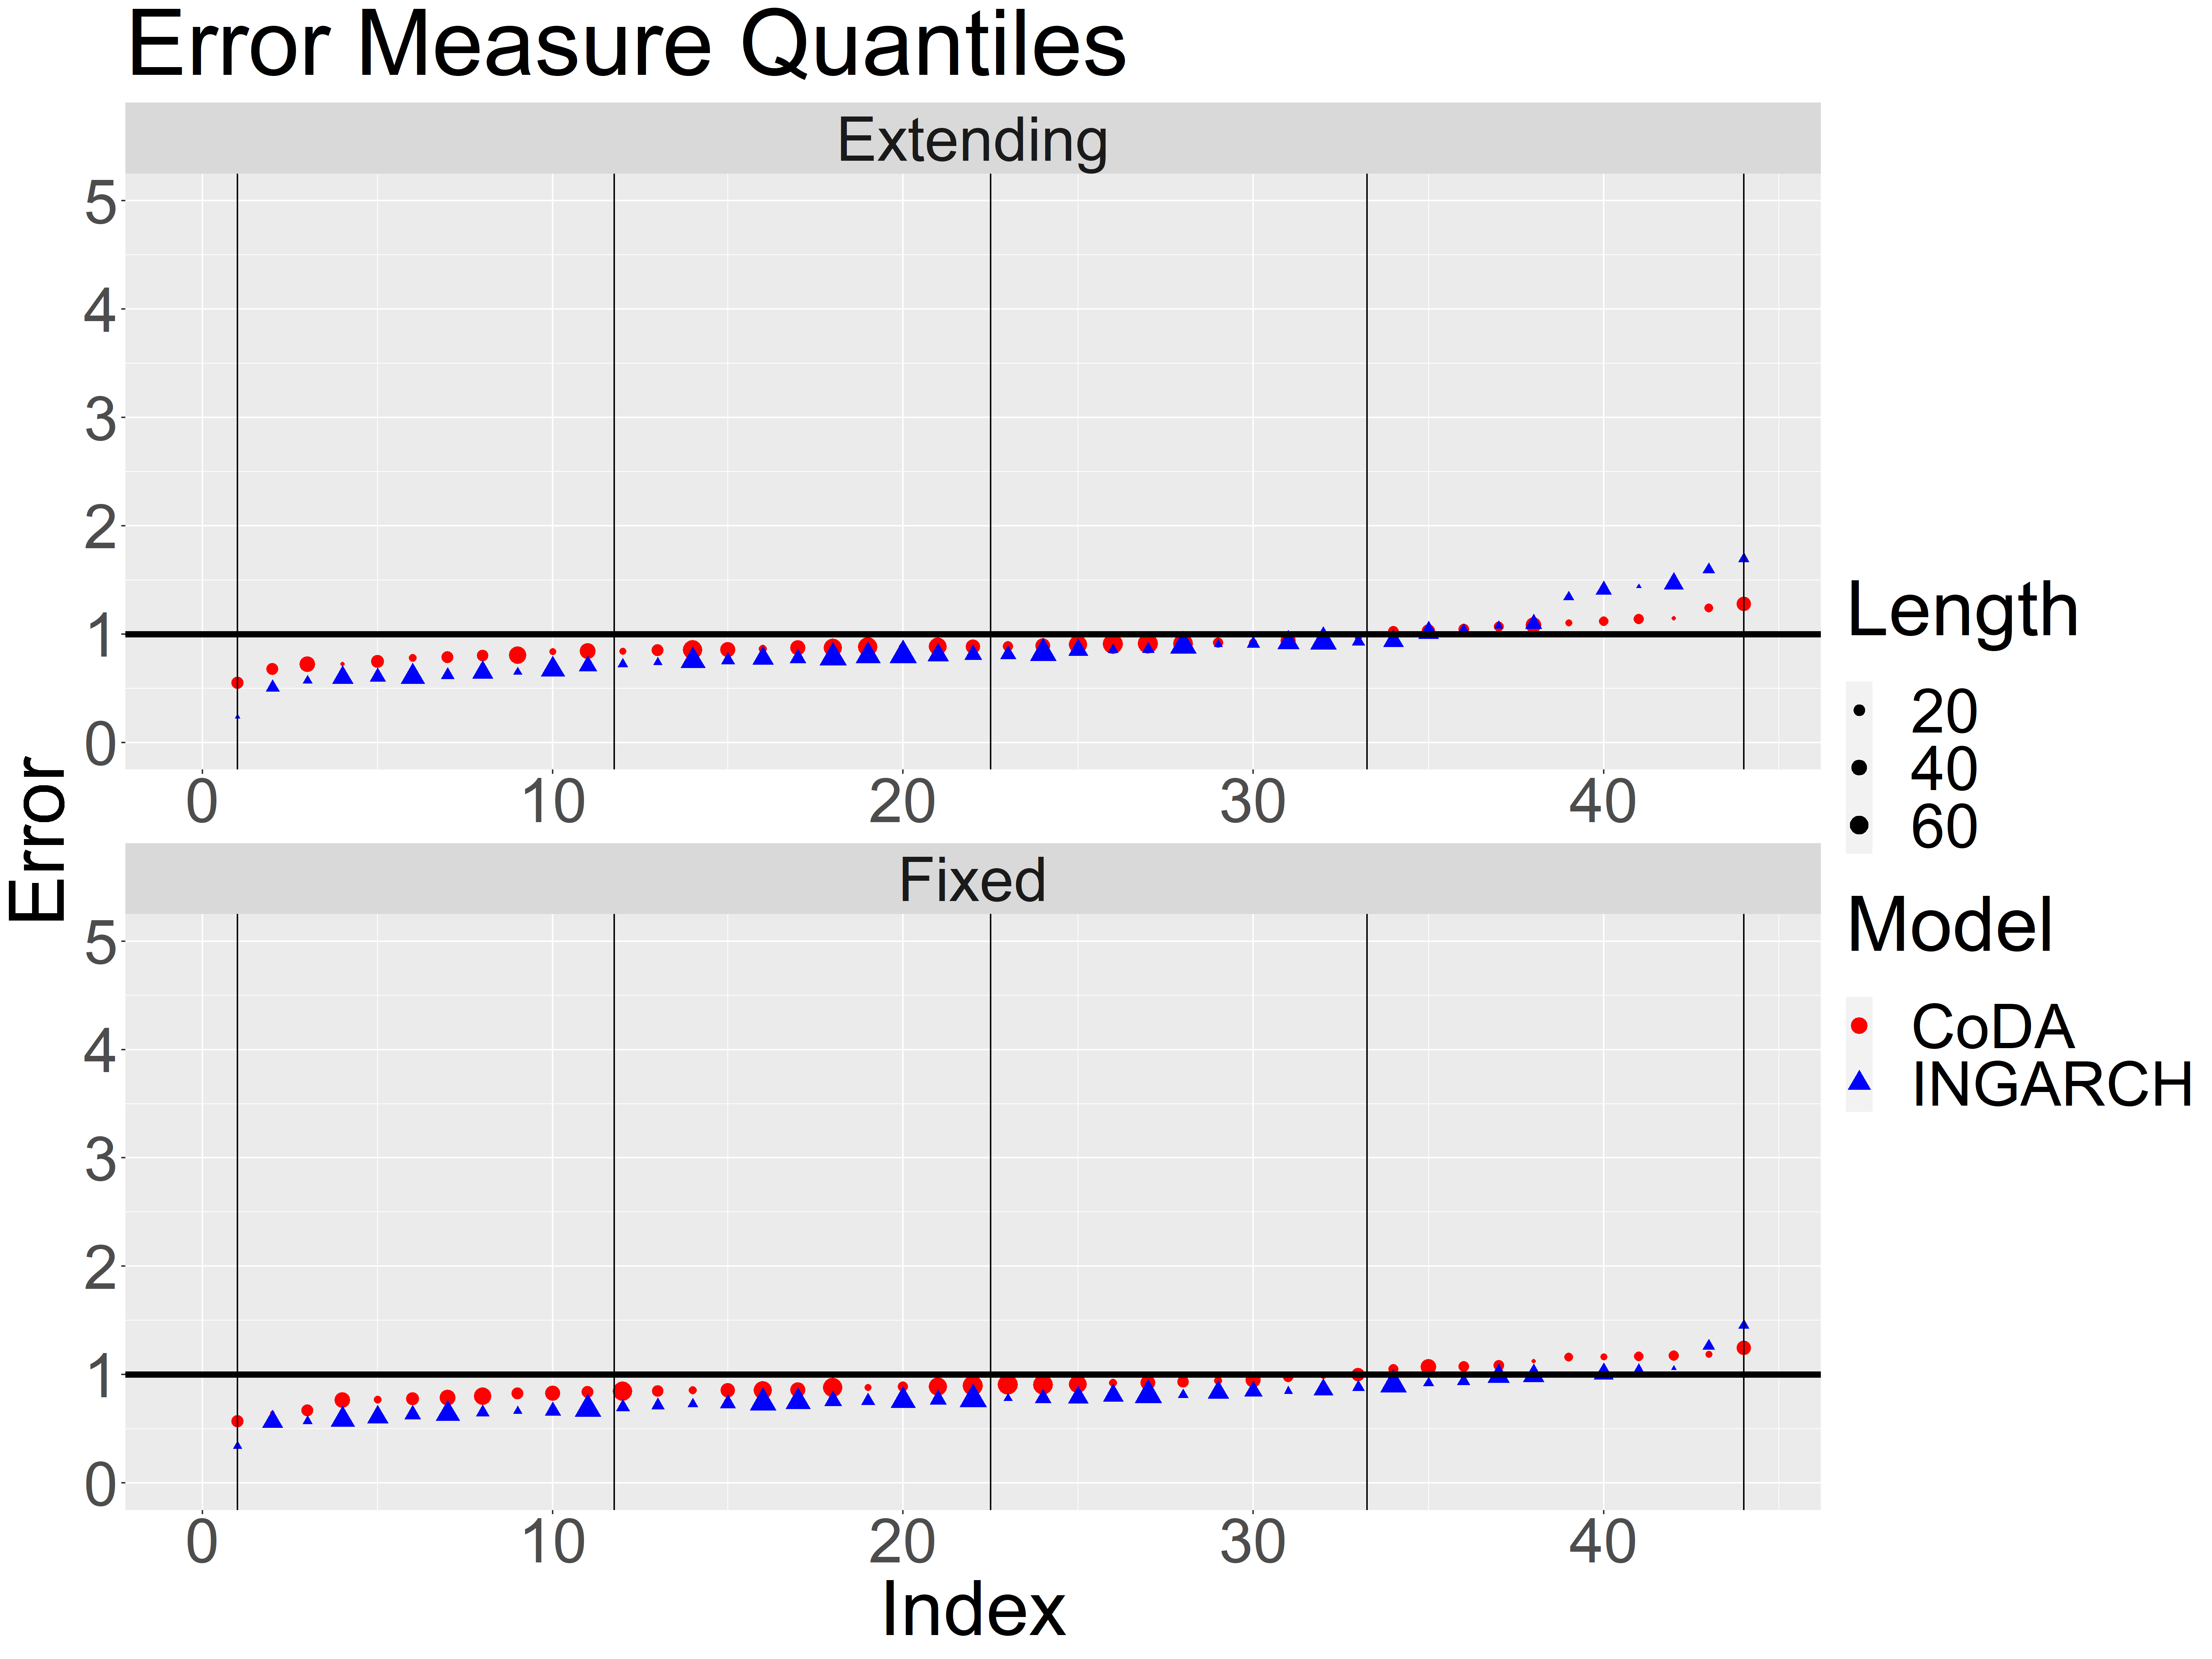
\includegraphics[width=\textwidth]{ErrorMeasureCombined_Quant_all__Variation_windowMethod.png}
\caption{Quantiles for different window shapes}
\label{fig:window methods Quant}
\end{subfigure}
\caption{Comparison of different window shapes}
\label{fig:window methods Comp1}
\end{figure}


\subsection{INGARCH Specifications}
\label{sec: Ingarch Specifications}

Next we will investigate the INGARCH specific options. 

\subsubsection{Distribution}
\label{sec:Distribution}

As mentioned in \ref{sec: Ingarch Specifications} we can replace the Poisson distribution with a Negative Binomial Distribution in \ref{eq:Ingarch Distribution}. The results are shown in \ref{fig:distributions Comp1}. 

\begin{figure}[htb!]
\centering
\begin{subfigure}[b]{0.45\textwidth}
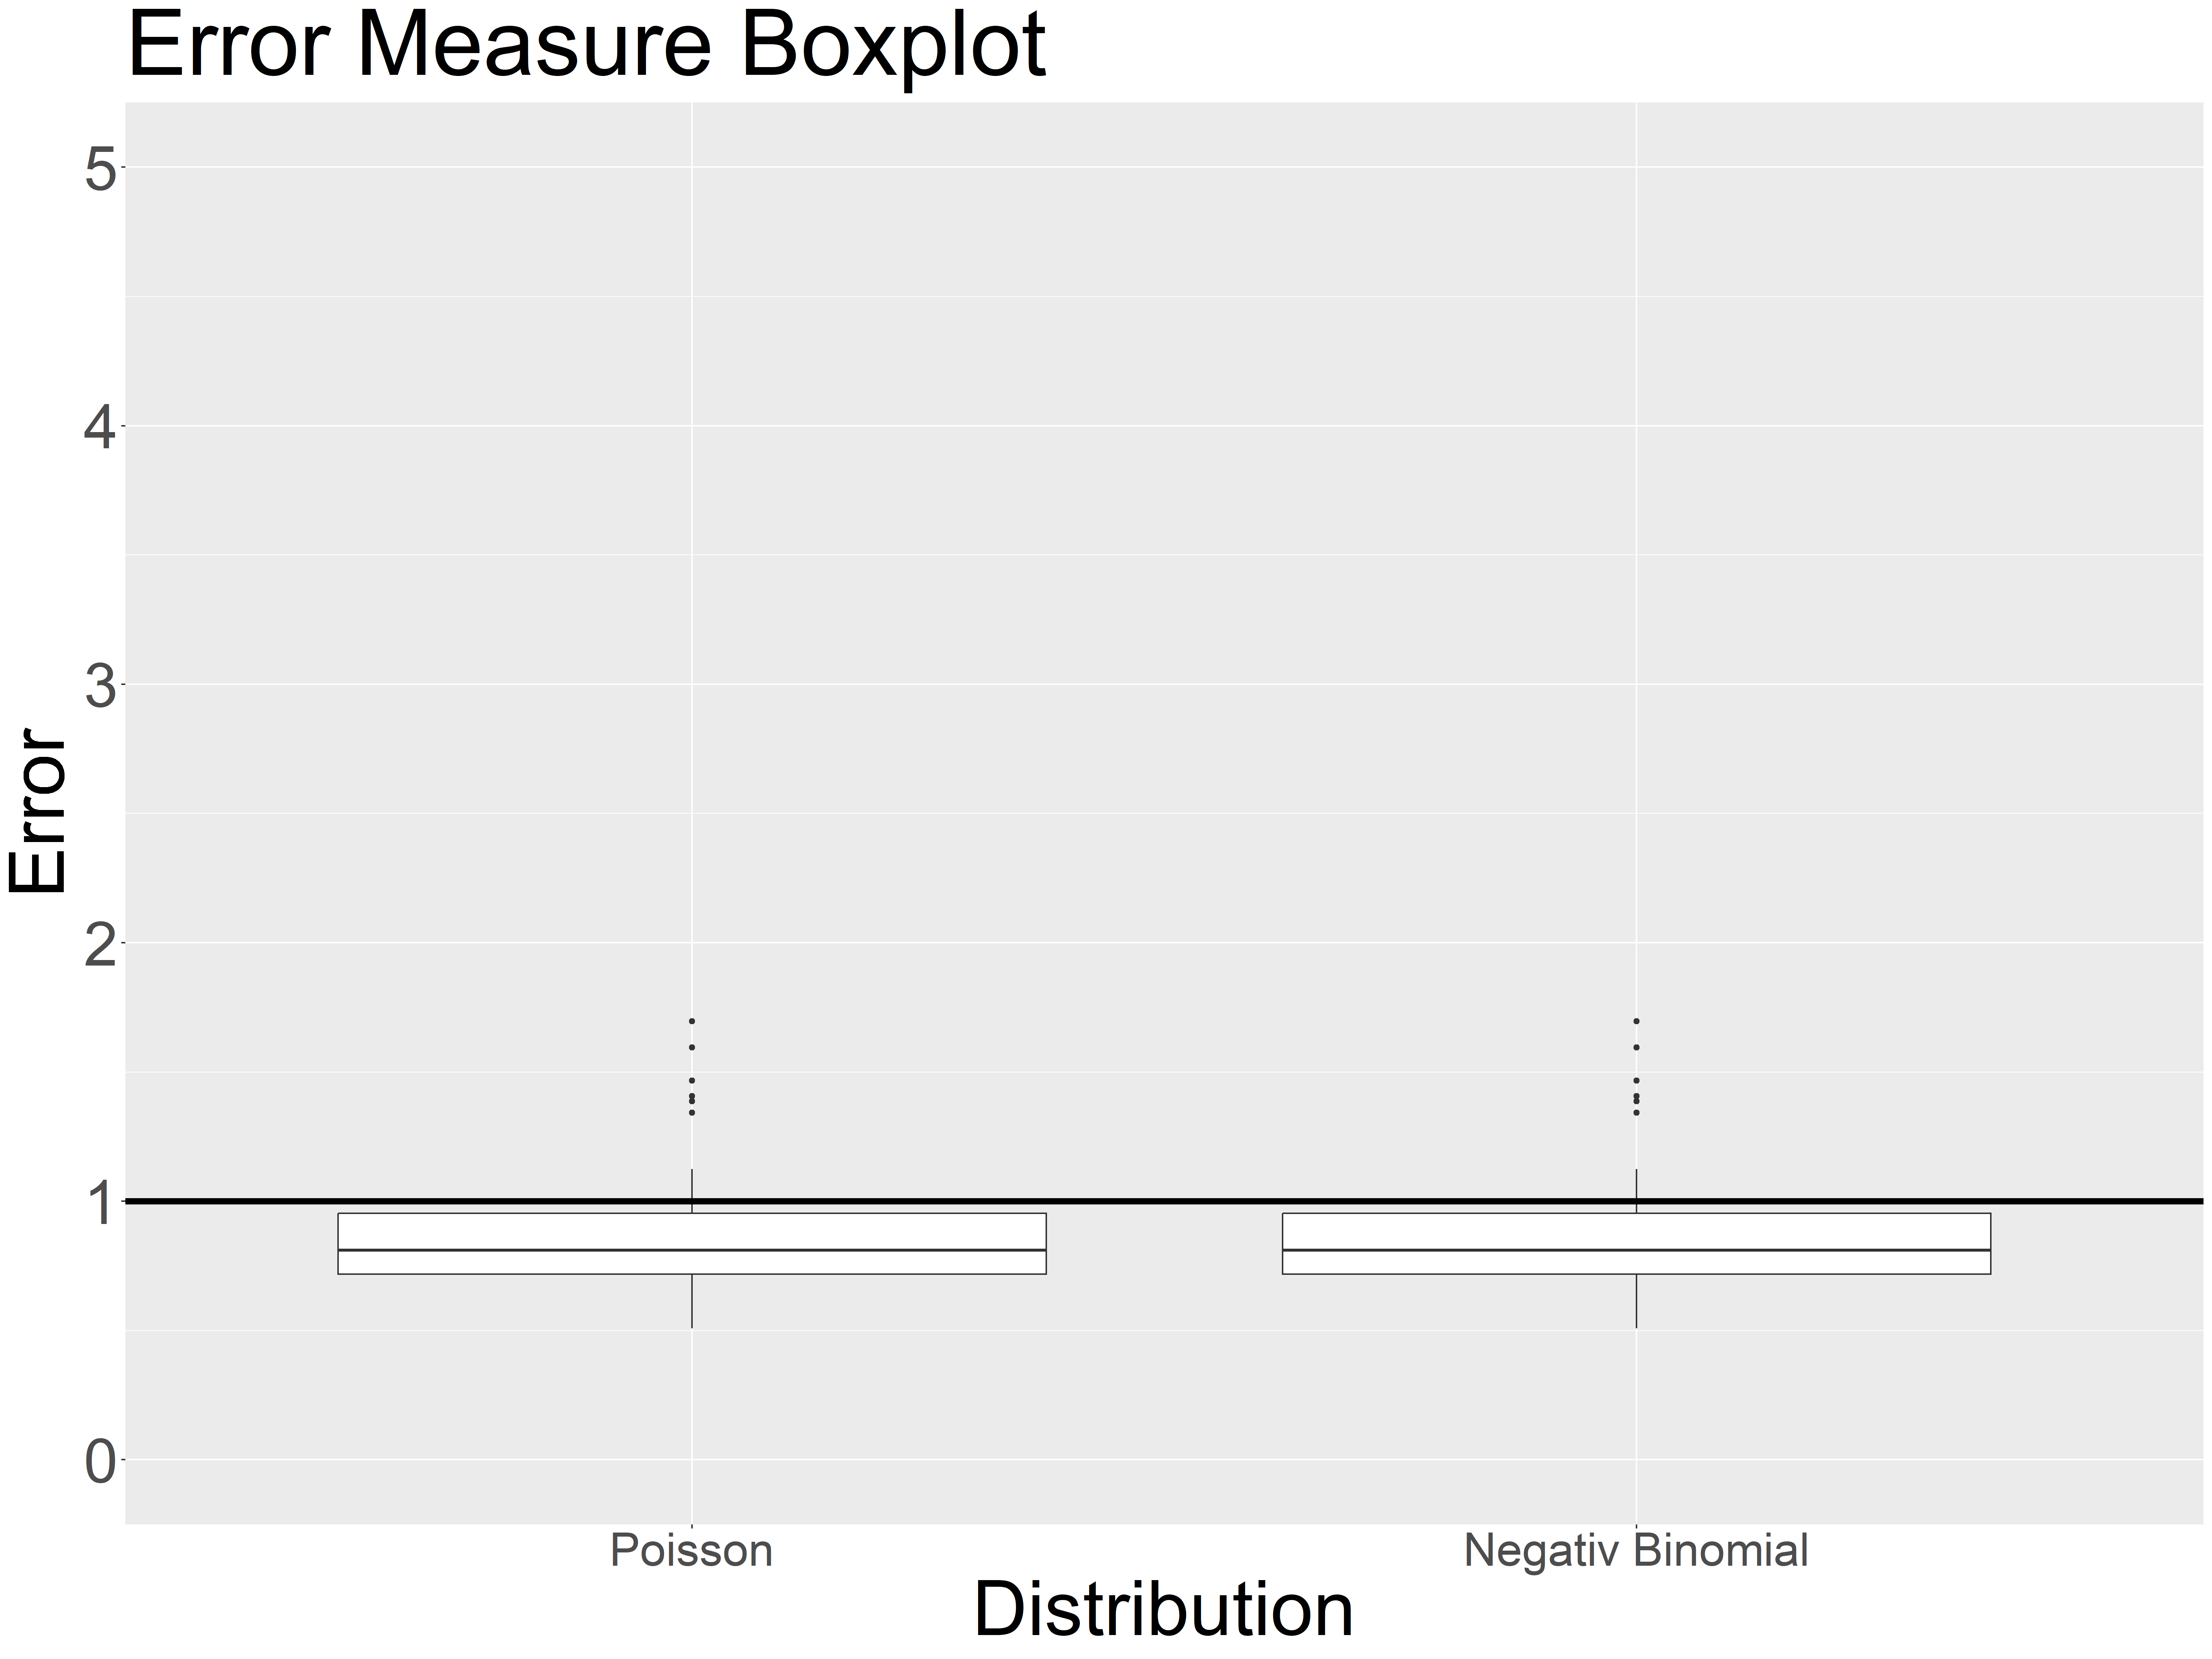
\includegraphics[width=\textwidth]{ErrorMeasureINGARCH_Box_all__Variation_distribution.png}
\caption{Boxplot for different distributions}
\label{fig:distributions Box}
\end{subfigure}
\hfill
\begin{subfigure}[b]{0.45\textwidth}
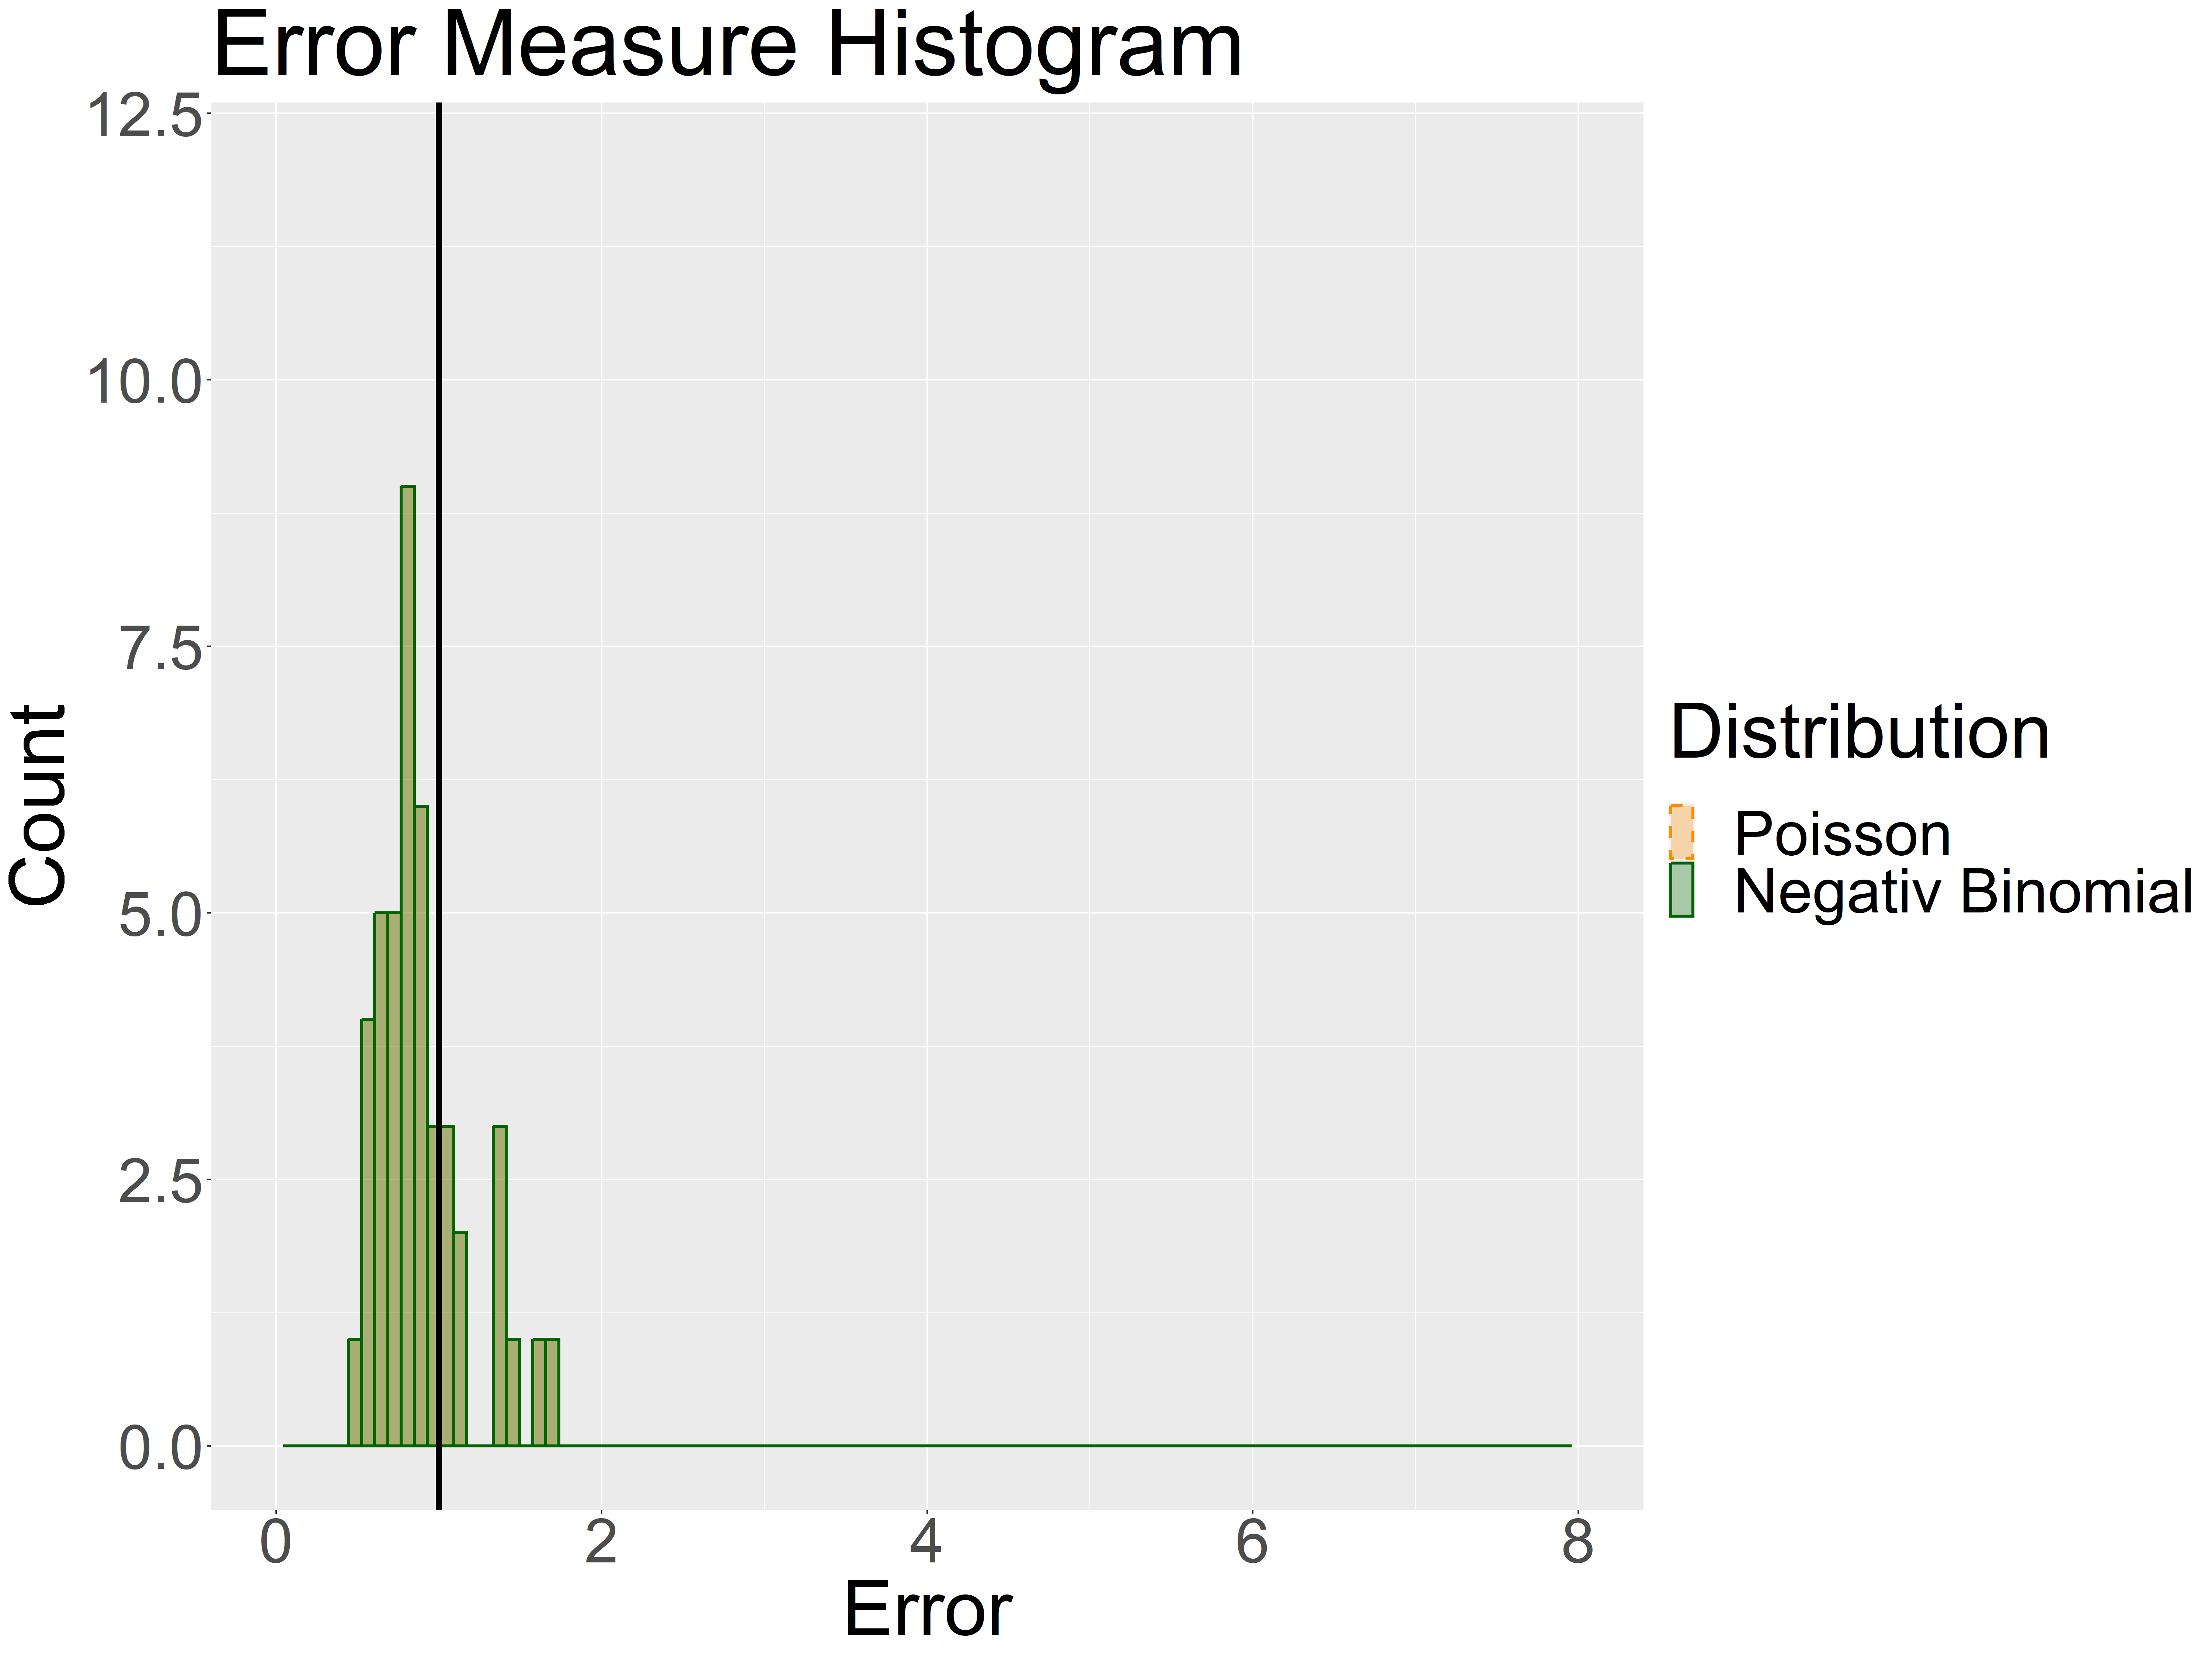
\includegraphics[width=\textwidth]{ErrorMeasureINGARCH_Histogram_all__Variation_distribution.png}
\caption{Histogram for different distributions}
\label{fig:distributions Hist}
\end{subfigure}
\hfill
%\begin{subfigure}[b]{0.8\textwidth}
%\includegraphics[width=\textwidth]{ErrorMeasureINGARCH_Quant_all__Variation_windowMethod.png}
%\caption{Quantiles for different distributions}
%\label{fig:window methods Quant}
%\end{subfigure}
\caption{Comparison of different distributions}
\label{fig:distributions Comp1}
\end{figure}

As we can see, we get the exactly the same results for both distributions. Since the Poisson Distribution is a limiting case of the Negative Binomial Distribution when $\phi \longrightarrow \infty$ in \ref{eq:Ingarch negbinom Distribution}, \cite{Liboschik:2016}. 


\subsubsection{Number of Past Means and Observations}
\label{sec: Number of Past Means and Observations}

The order in the INGARCH(p,q) model is another parameter which can be chosen. For simplicities sake we only compare our INGARCH(1,1) with an INGARCH(1,2) and INGARCH(2,1) model. However, further models could be tried out and compared. One could even optimise over the optimal order. 

In figure \ref{fig:past means Comp1} we compare the INGARCH(1,1) model (red) with the INGARCH(1,2) model (blue). We can see that the performance is very similar . Hence we prefer the smaller model. 
\begin{figure}[htb!]
\centering
\begin{subfigure}[b]{0.45\textwidth}
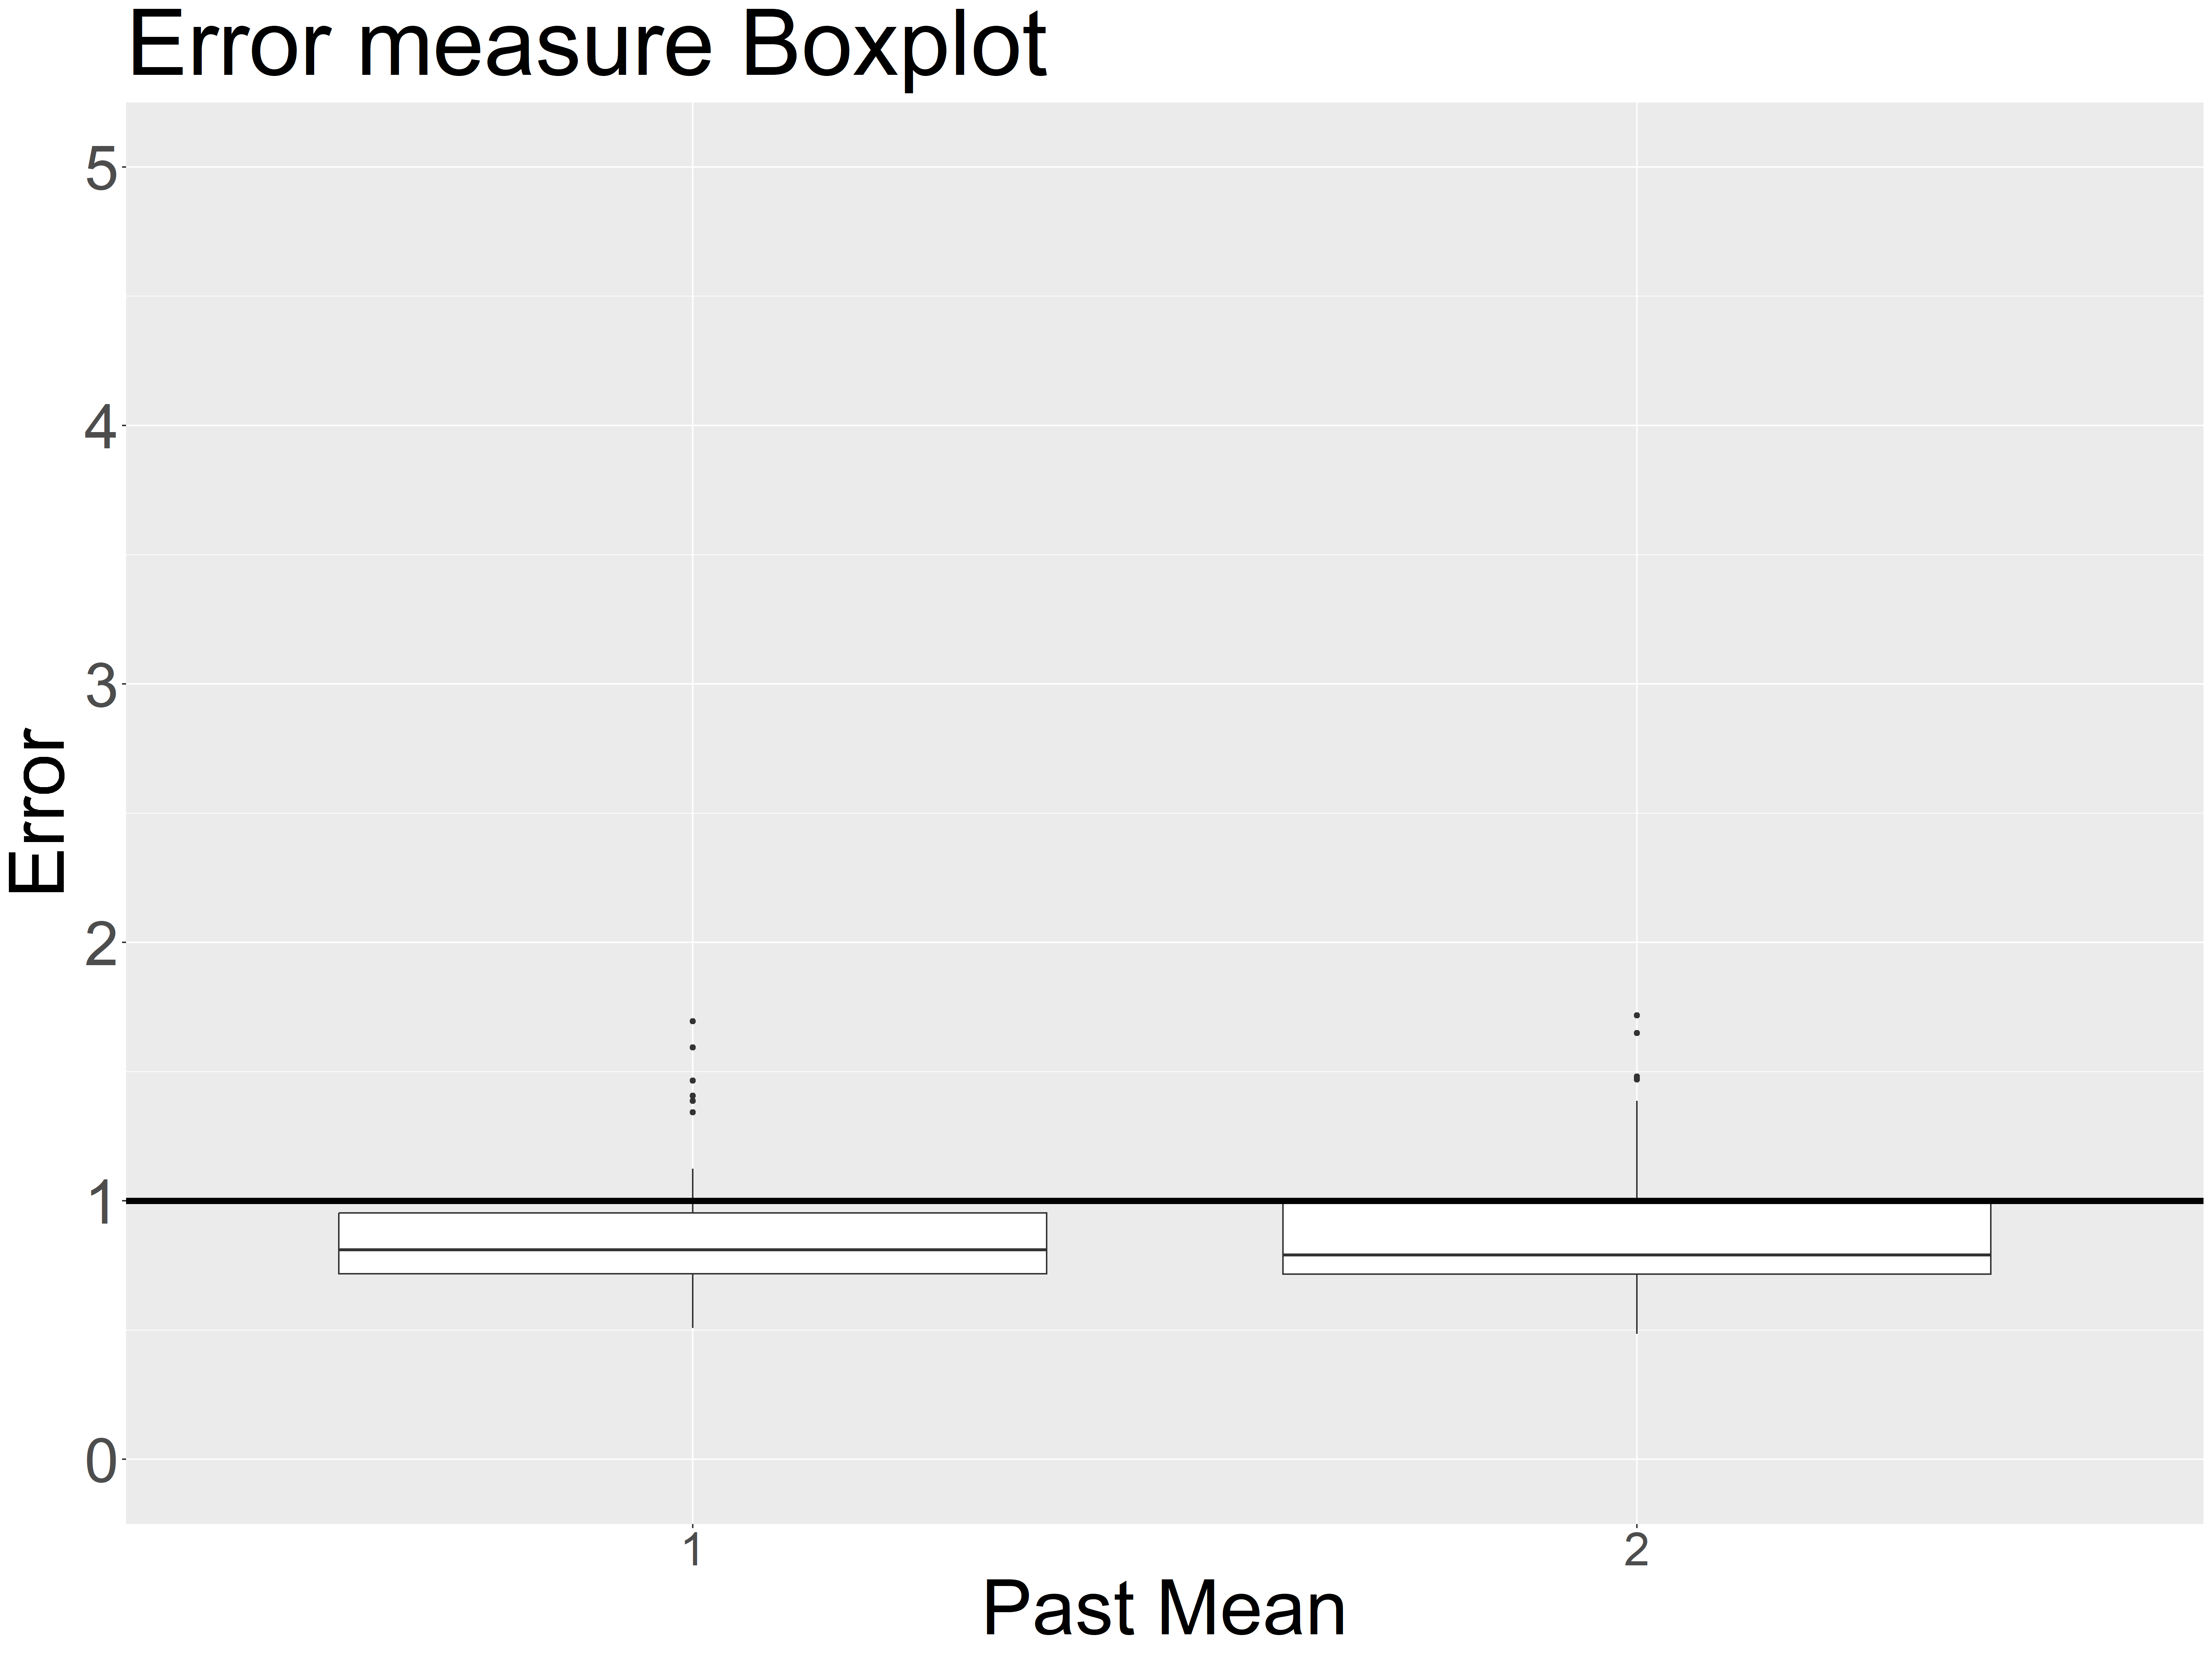
\includegraphics[width=\textwidth]{ErrorMeasureINGARCH_Box_all__Variation_pastMean.png}
\caption{Boxplot for a different number of past means}
\label{fig:past means Box}
\end{subfigure}
\hfill
\begin{subfigure}[b]{0.45\textwidth}
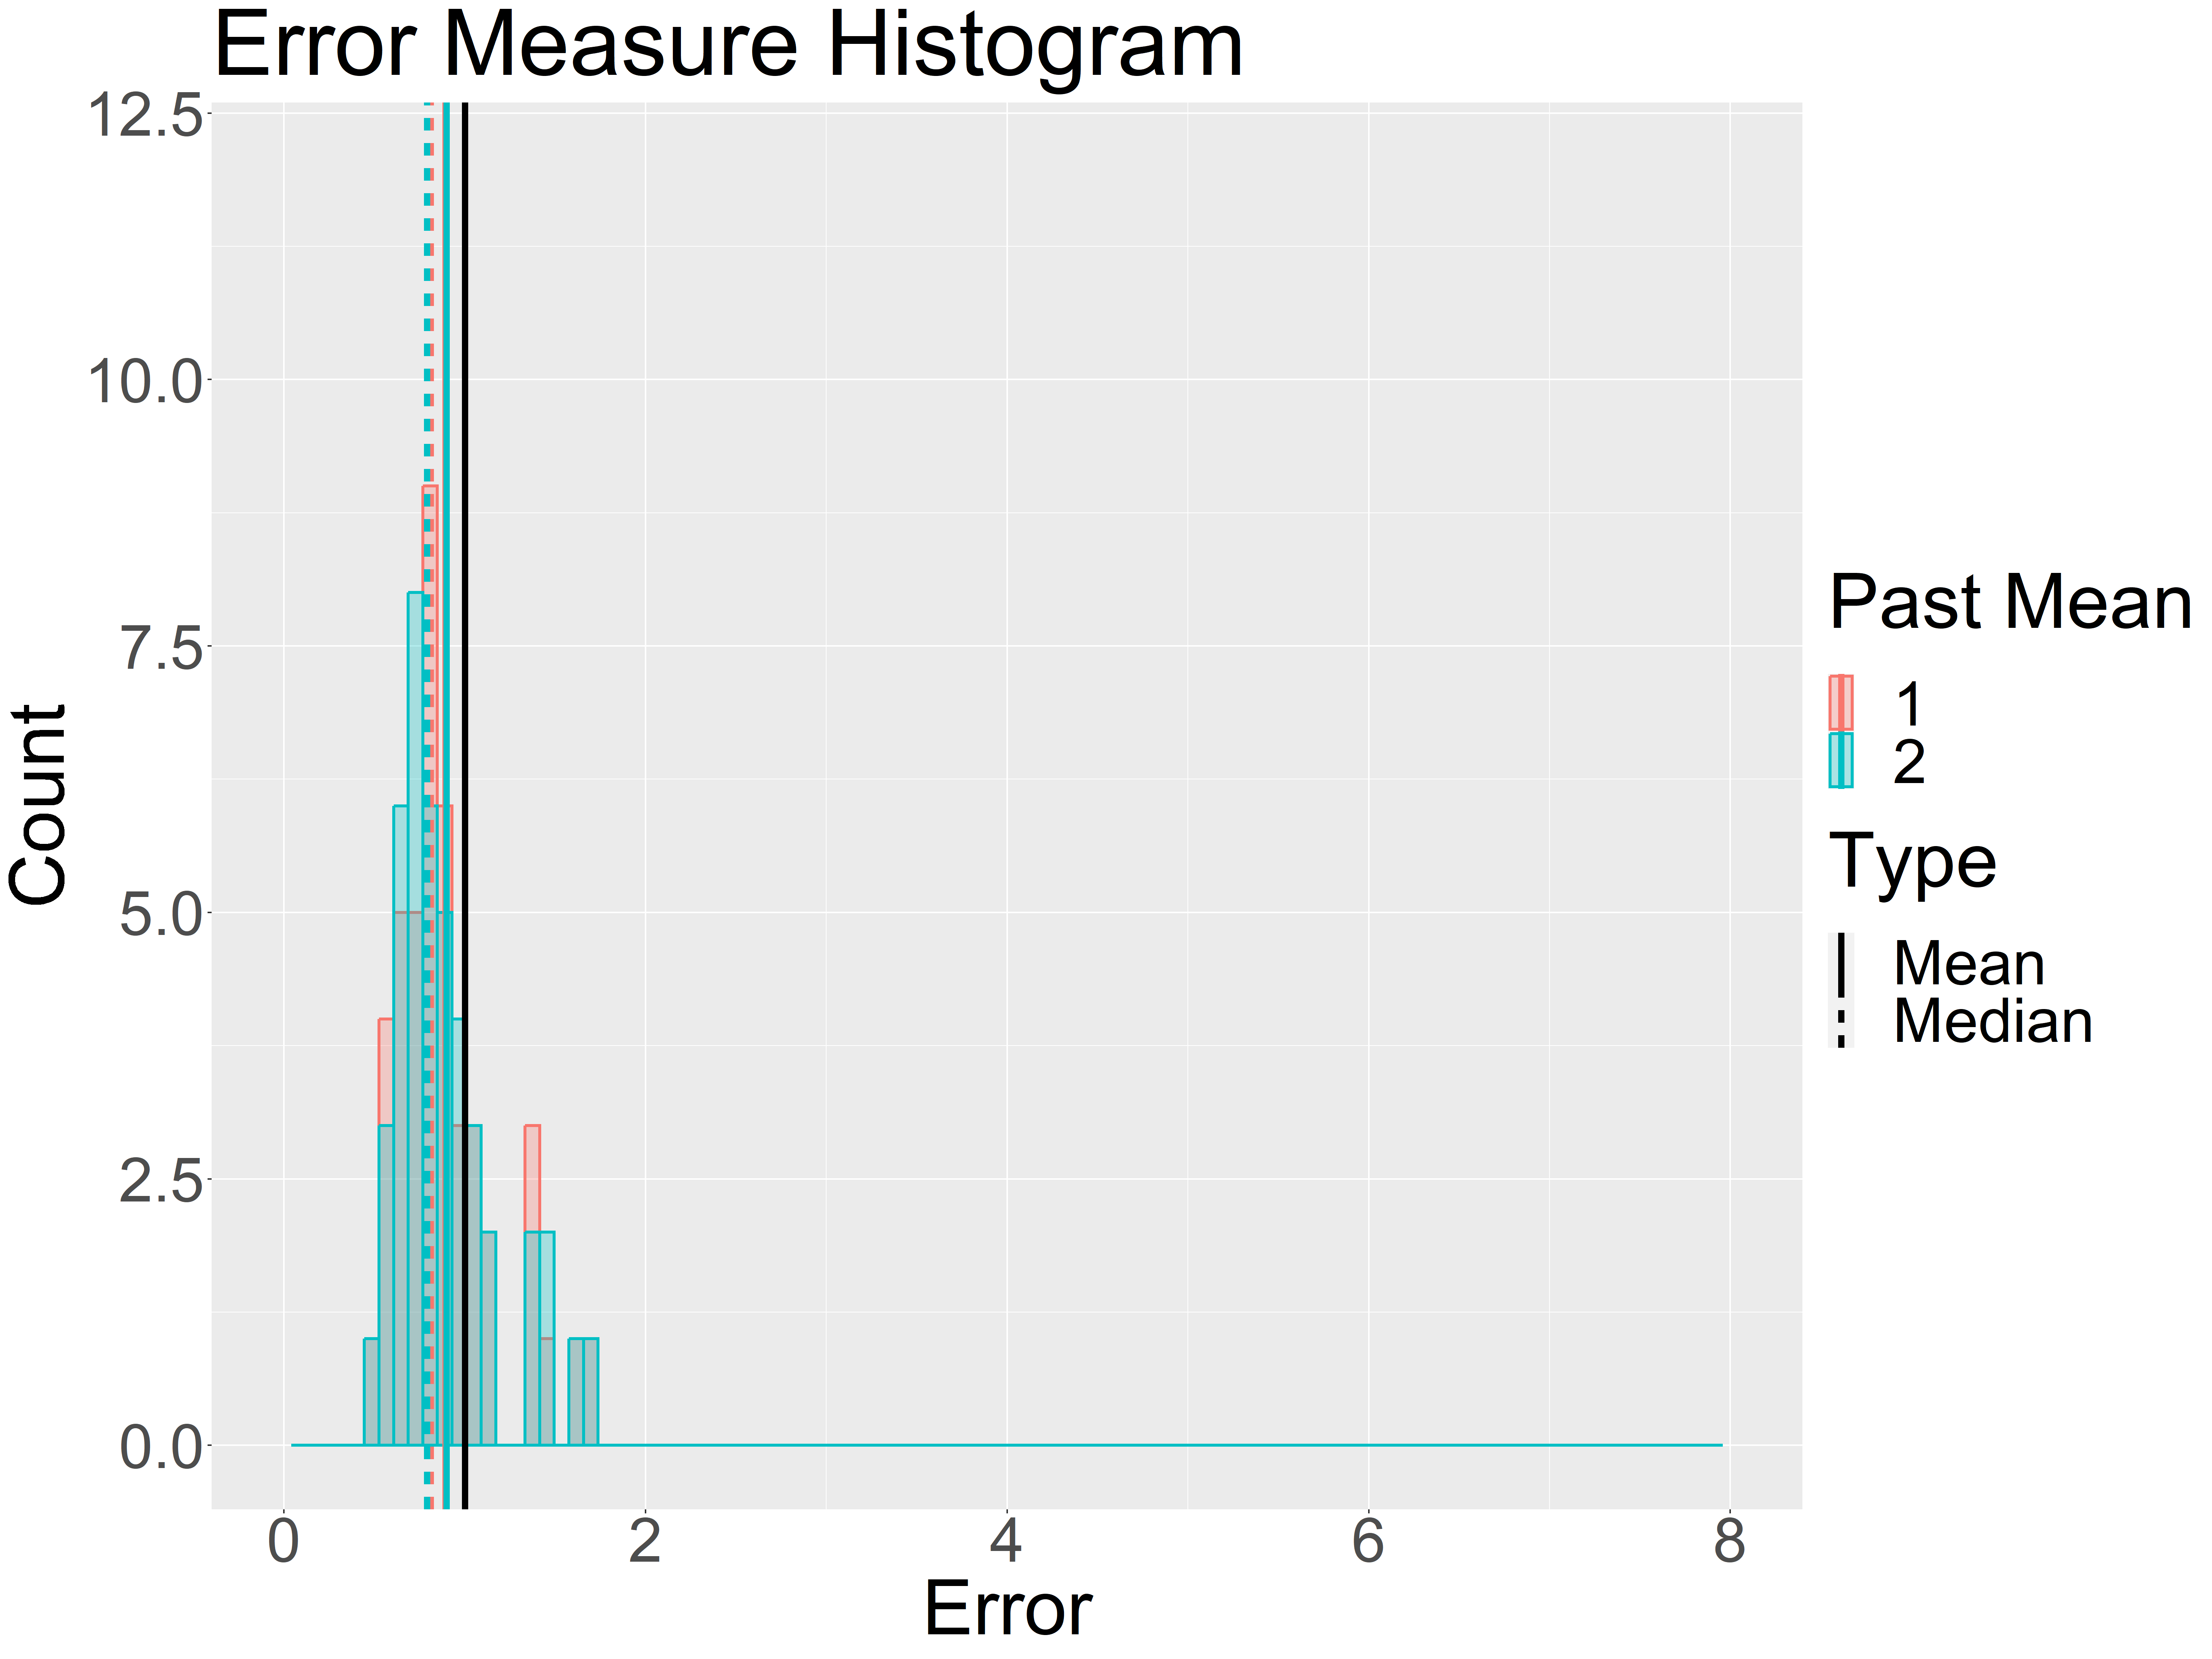
\includegraphics[width=\textwidth]{ErrorMeasureINGARCH_Histogram_all__Variation_pastMean.png}
\caption{Histogram for a different number of past means}
\label{fig:past means Hist}
\end{subfigure}
\hfill
\begin{subfigure}[b]{0.8\textwidth}
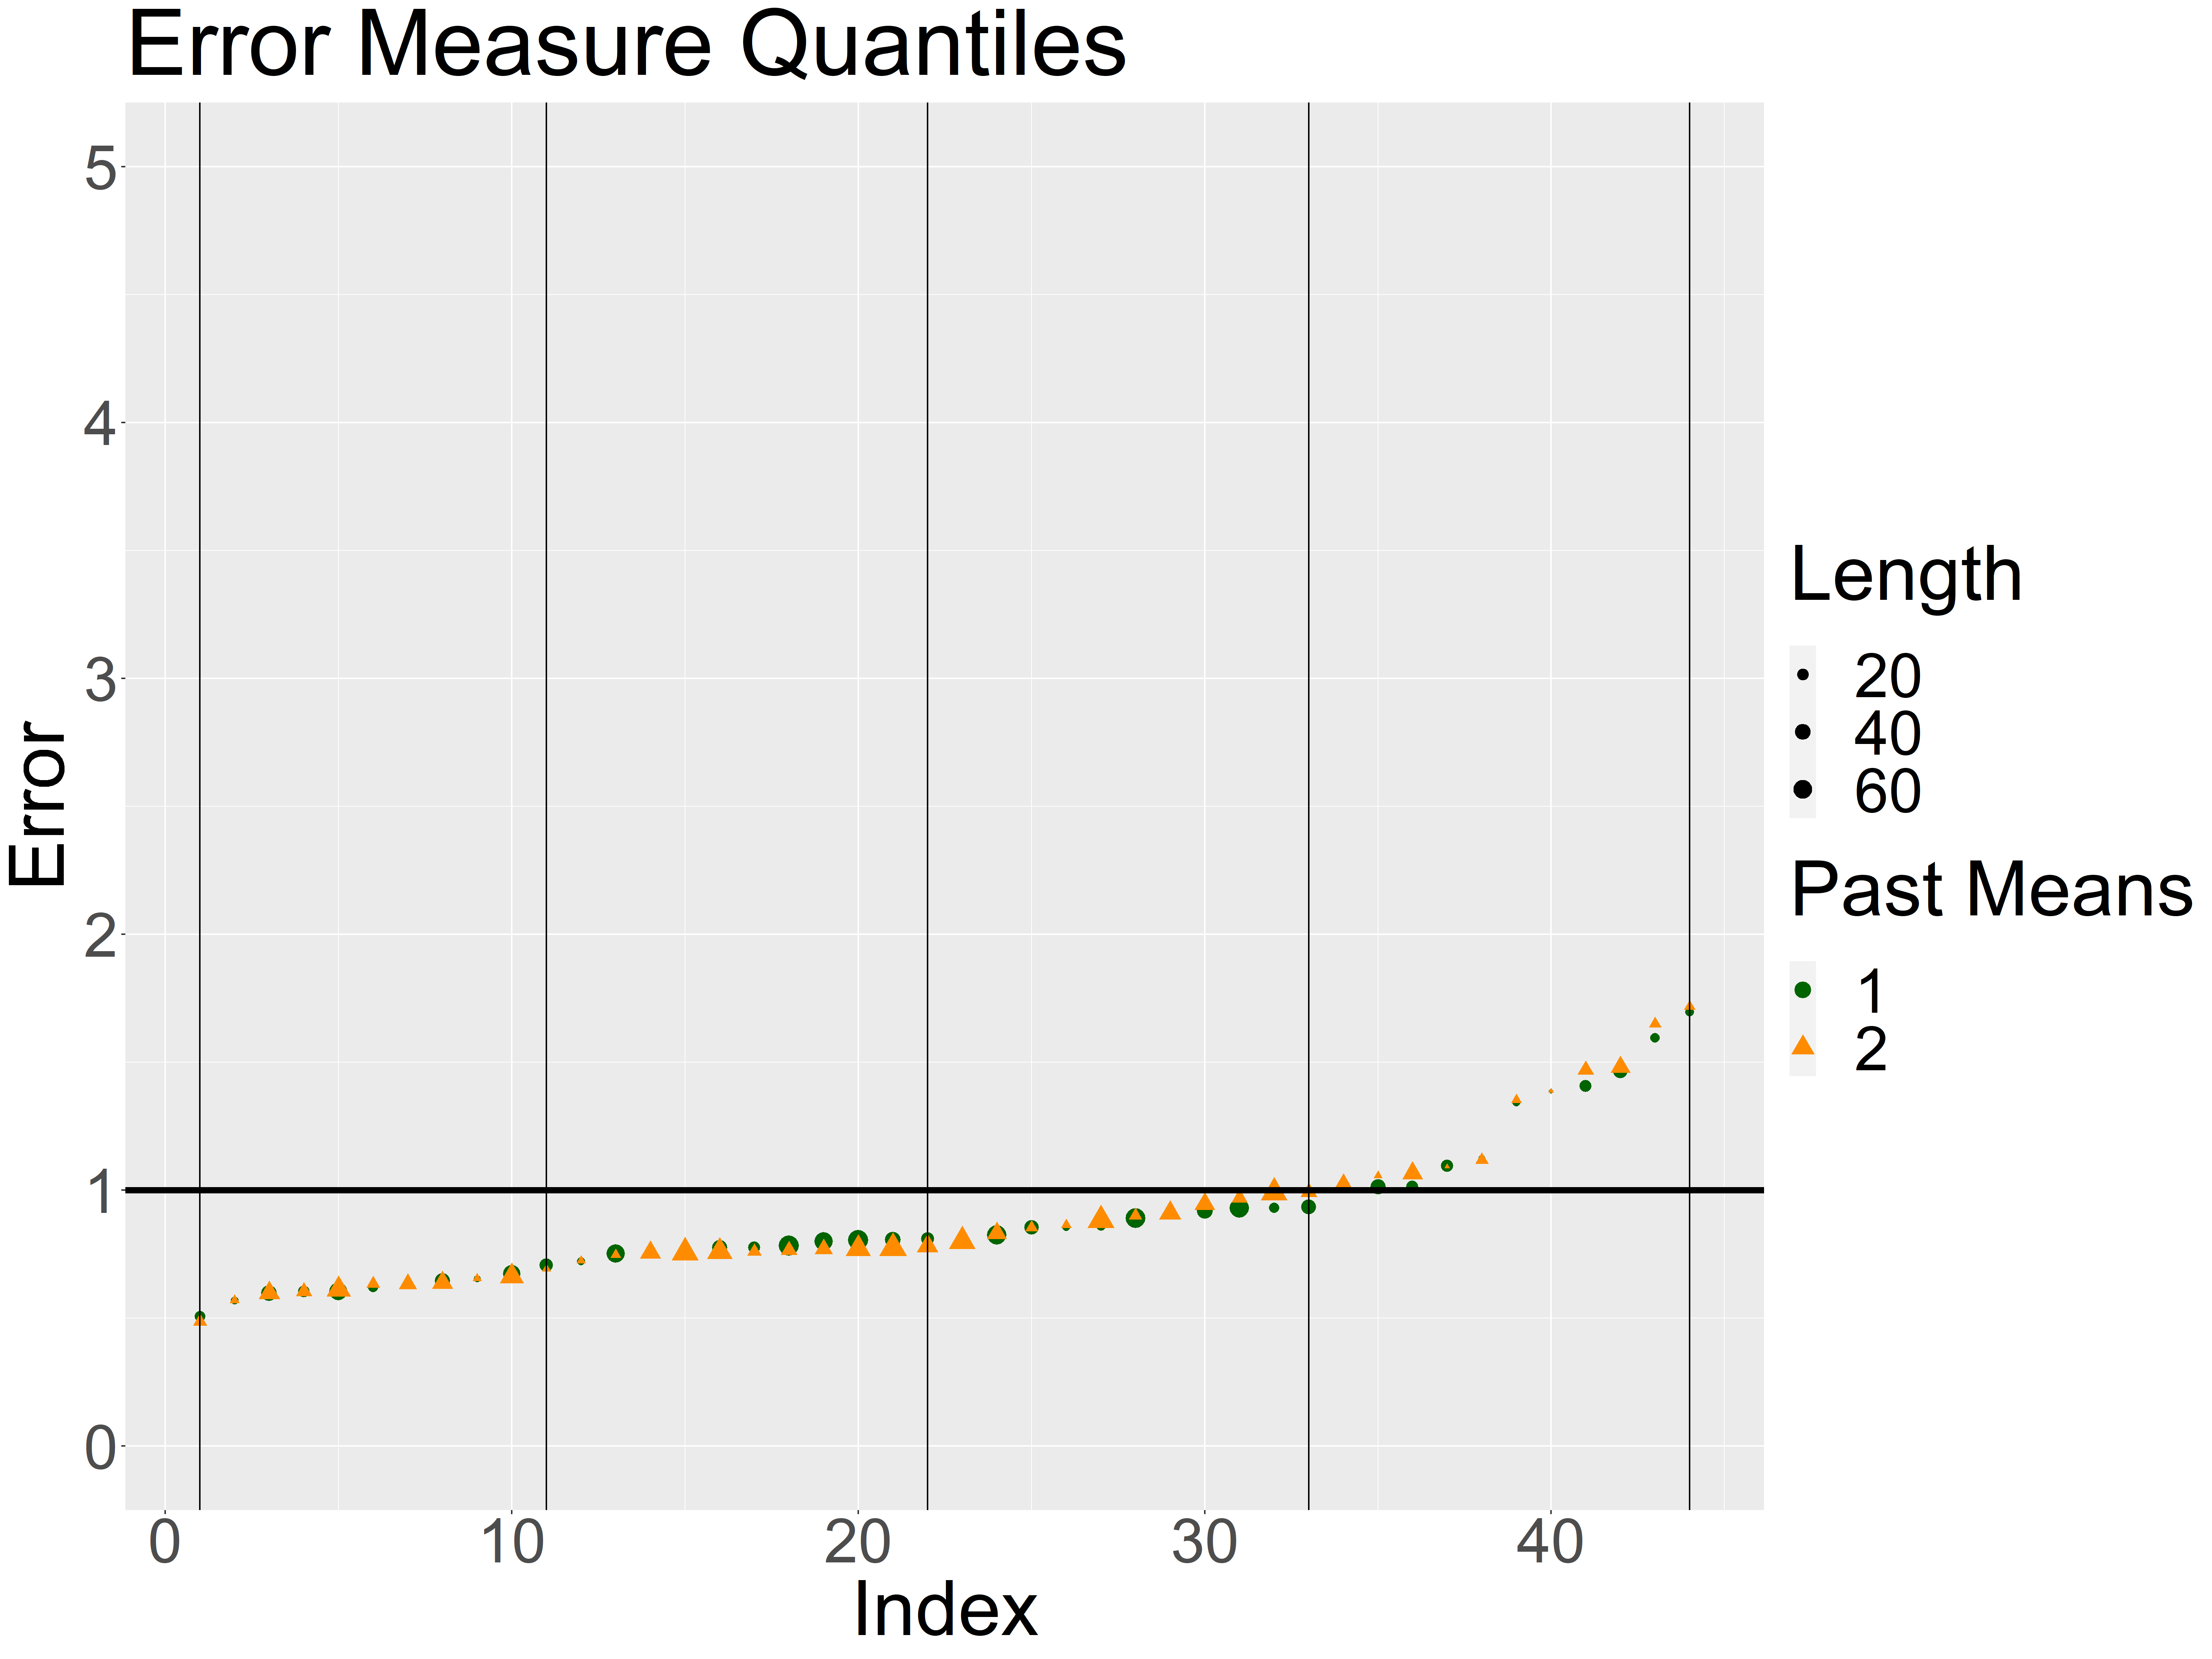
\includegraphics[width=\textwidth]{ErrorMeasureINGARCH_Quant_all__Variation_pastMean.png}
\caption{Quantiles for a different number of past means}
\label{fig:past means Quant}
\end{subfigure}
\caption{Comparison of a different number of past means}
\label{fig:past means Comp1}
\end{figure}


In figure \ref{fig:past obs Comp1} we compare the INGARCH(1,1) (red) model with the INGARCH(2,1) (blue) model. Again the performance is very similar in general. 

\begin{figure}[htb!]
\centering
\begin{subfigure}[b]{0.45\textwidth}
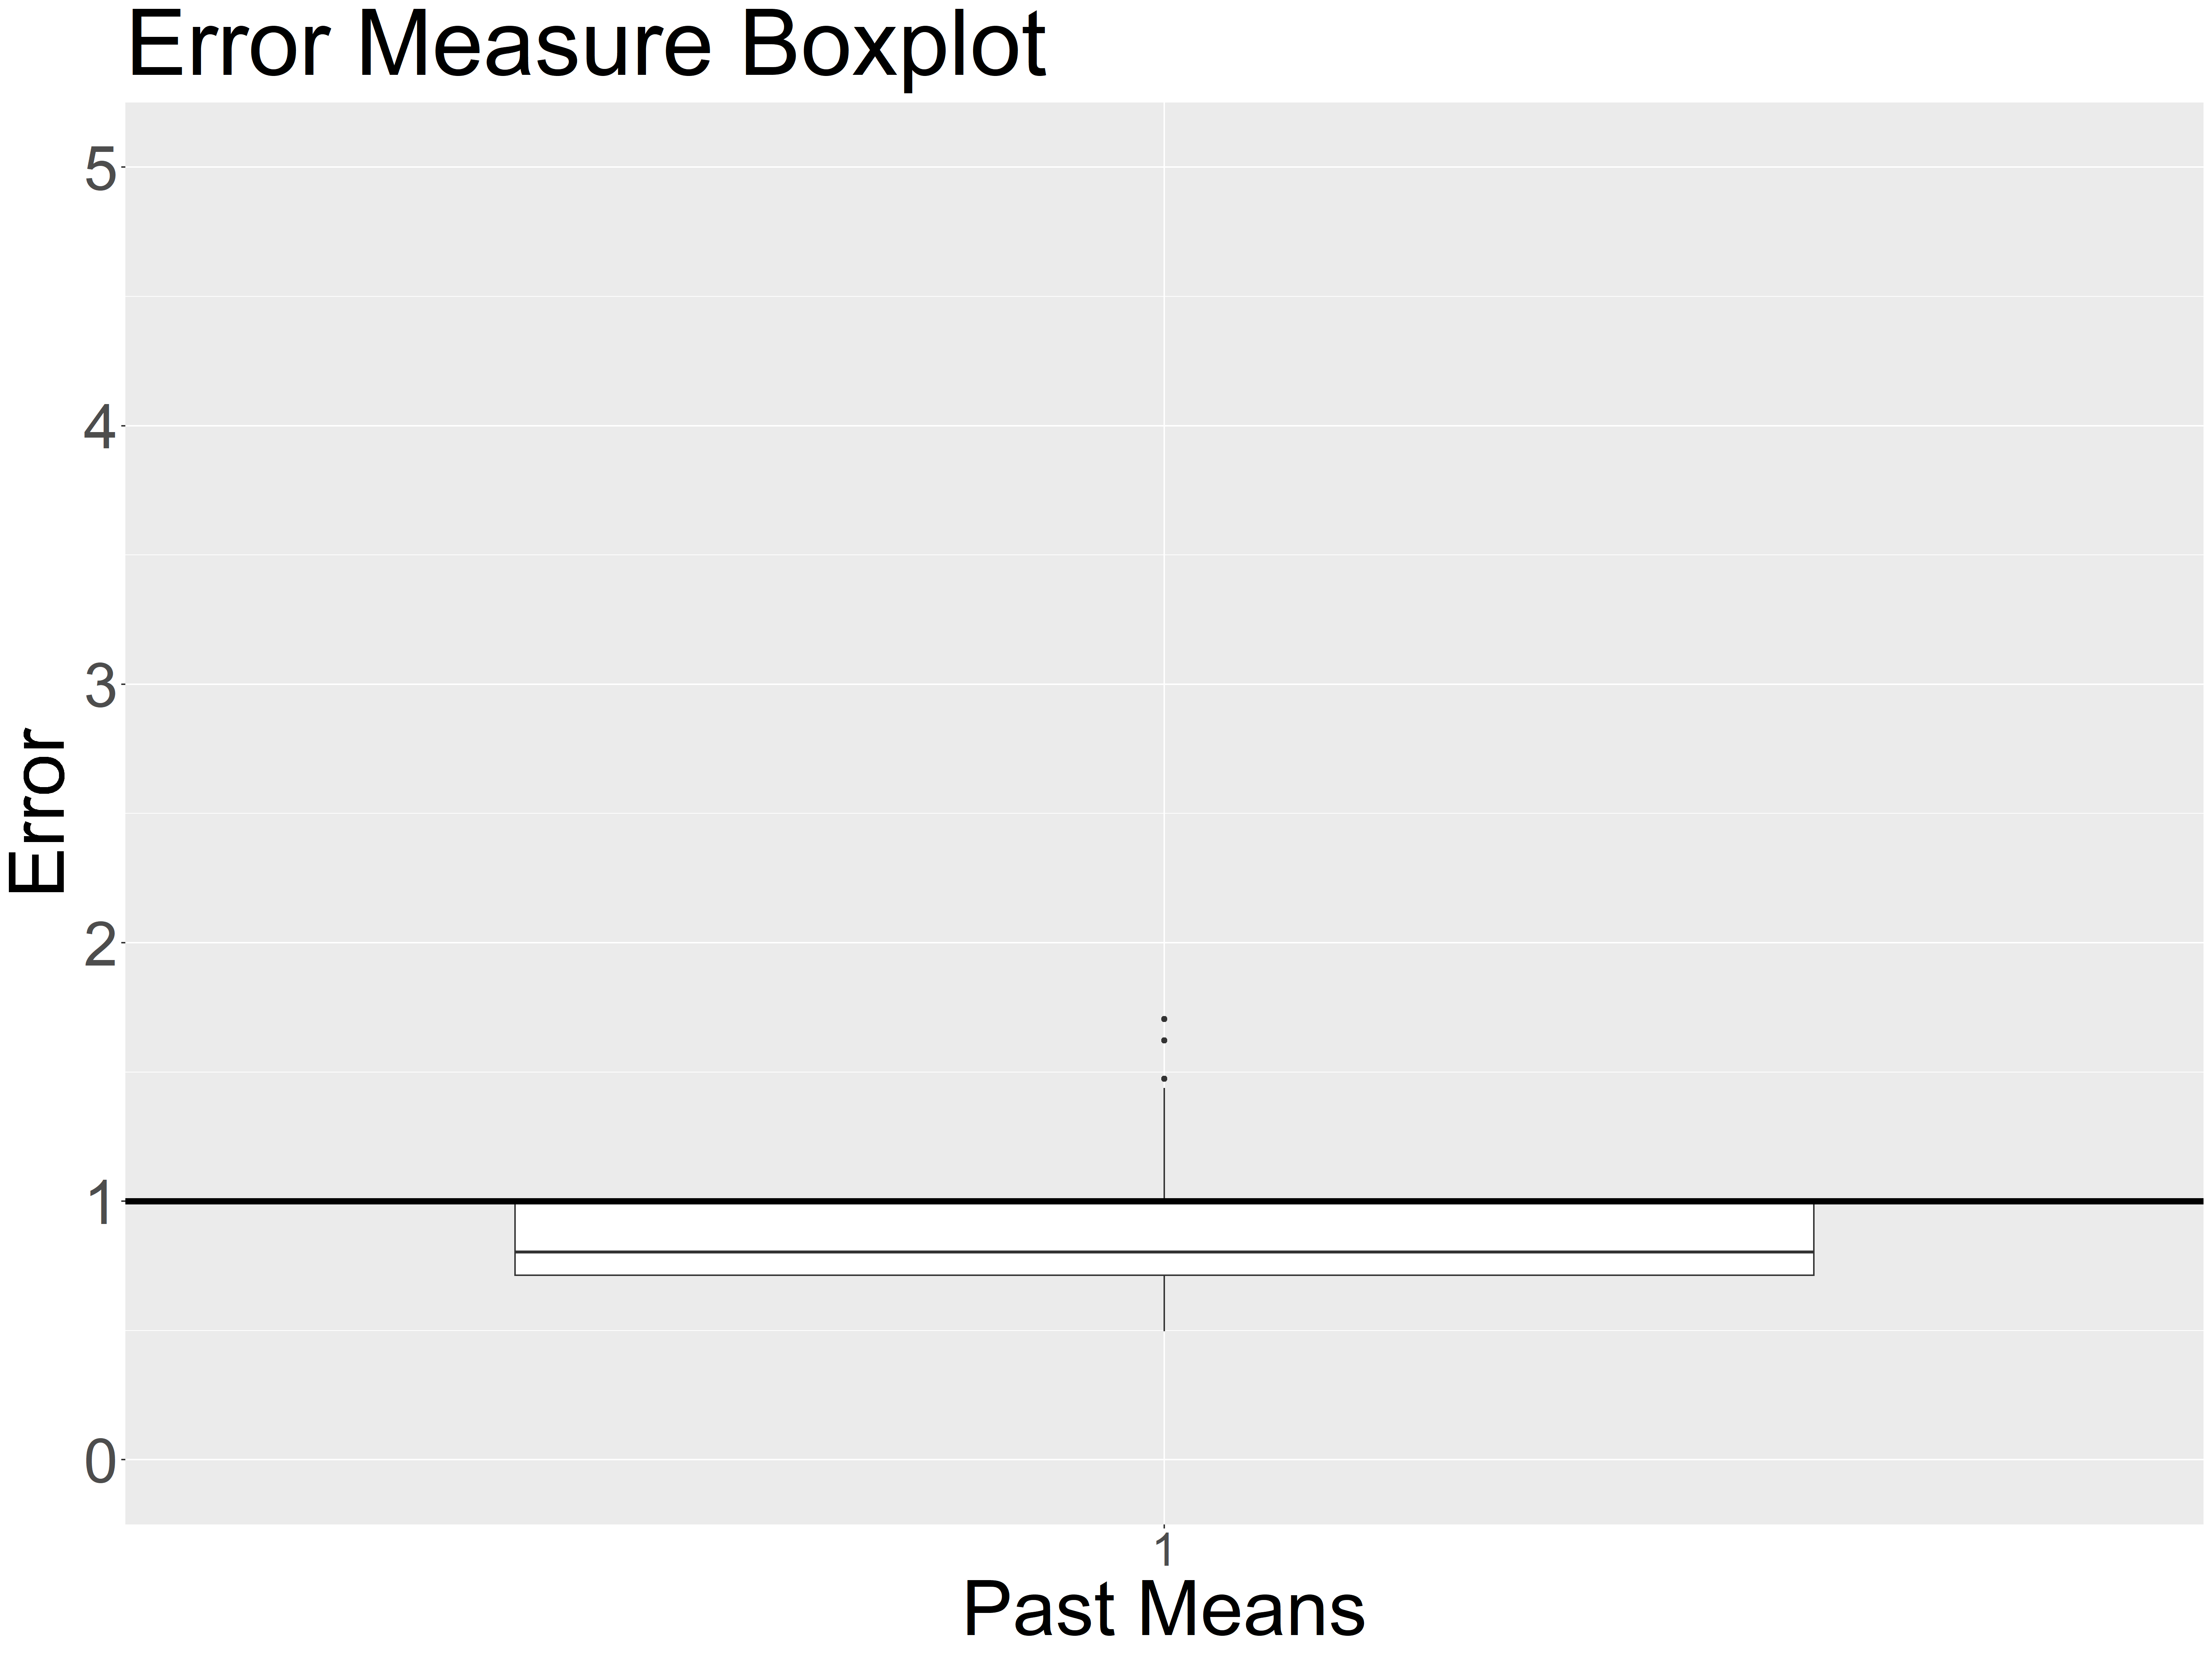
\includegraphics[width=\textwidth]{ErrorMeasureINGARCH_Box_all__Variation_pastOb.png}
\caption{Boxplot for a different number of past observations}
\label{fig:past obs Box}
\end{subfigure}
\hfill
\begin{subfigure}[b]{0.45\textwidth}
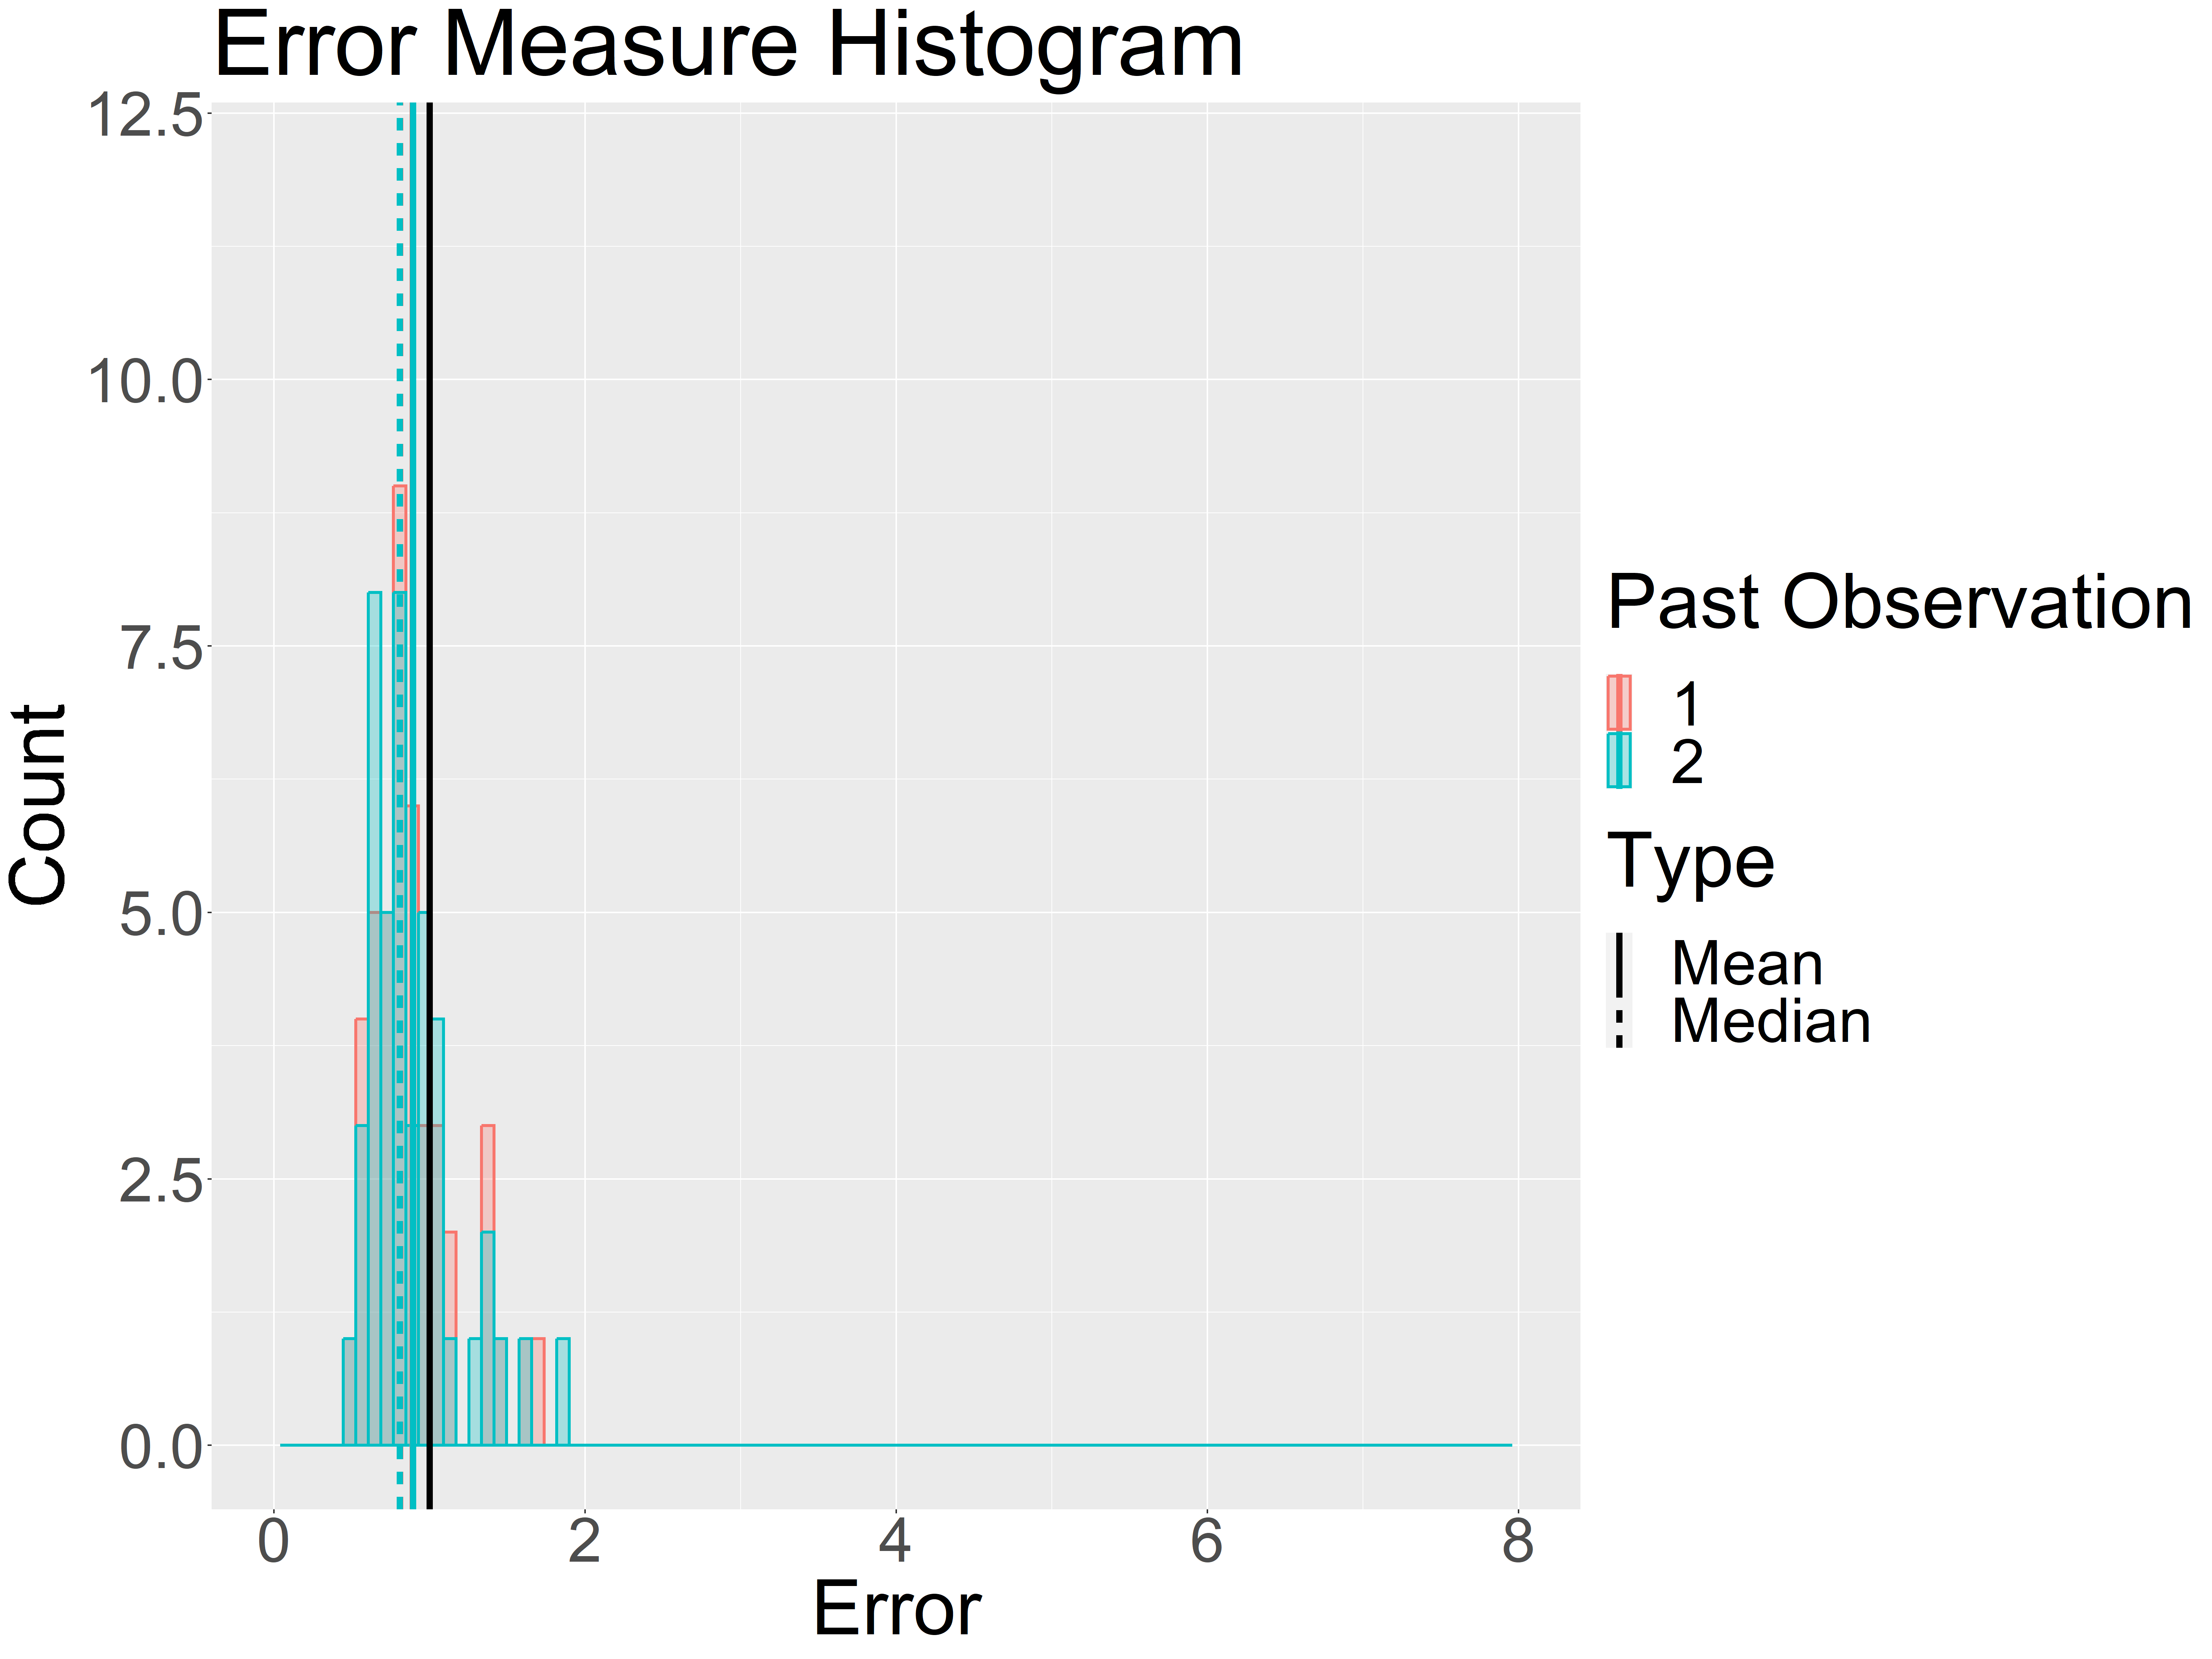
\includegraphics[width=\textwidth]{ErrorMeasureINGARCH_Histogram_all__Variation_pastOb.png}
\caption{Histogram for a different number of past observations}
\label{fig:past obs Hist}
\end{subfigure}
\hfill
\begin{subfigure}[b]{0.8\textwidth}
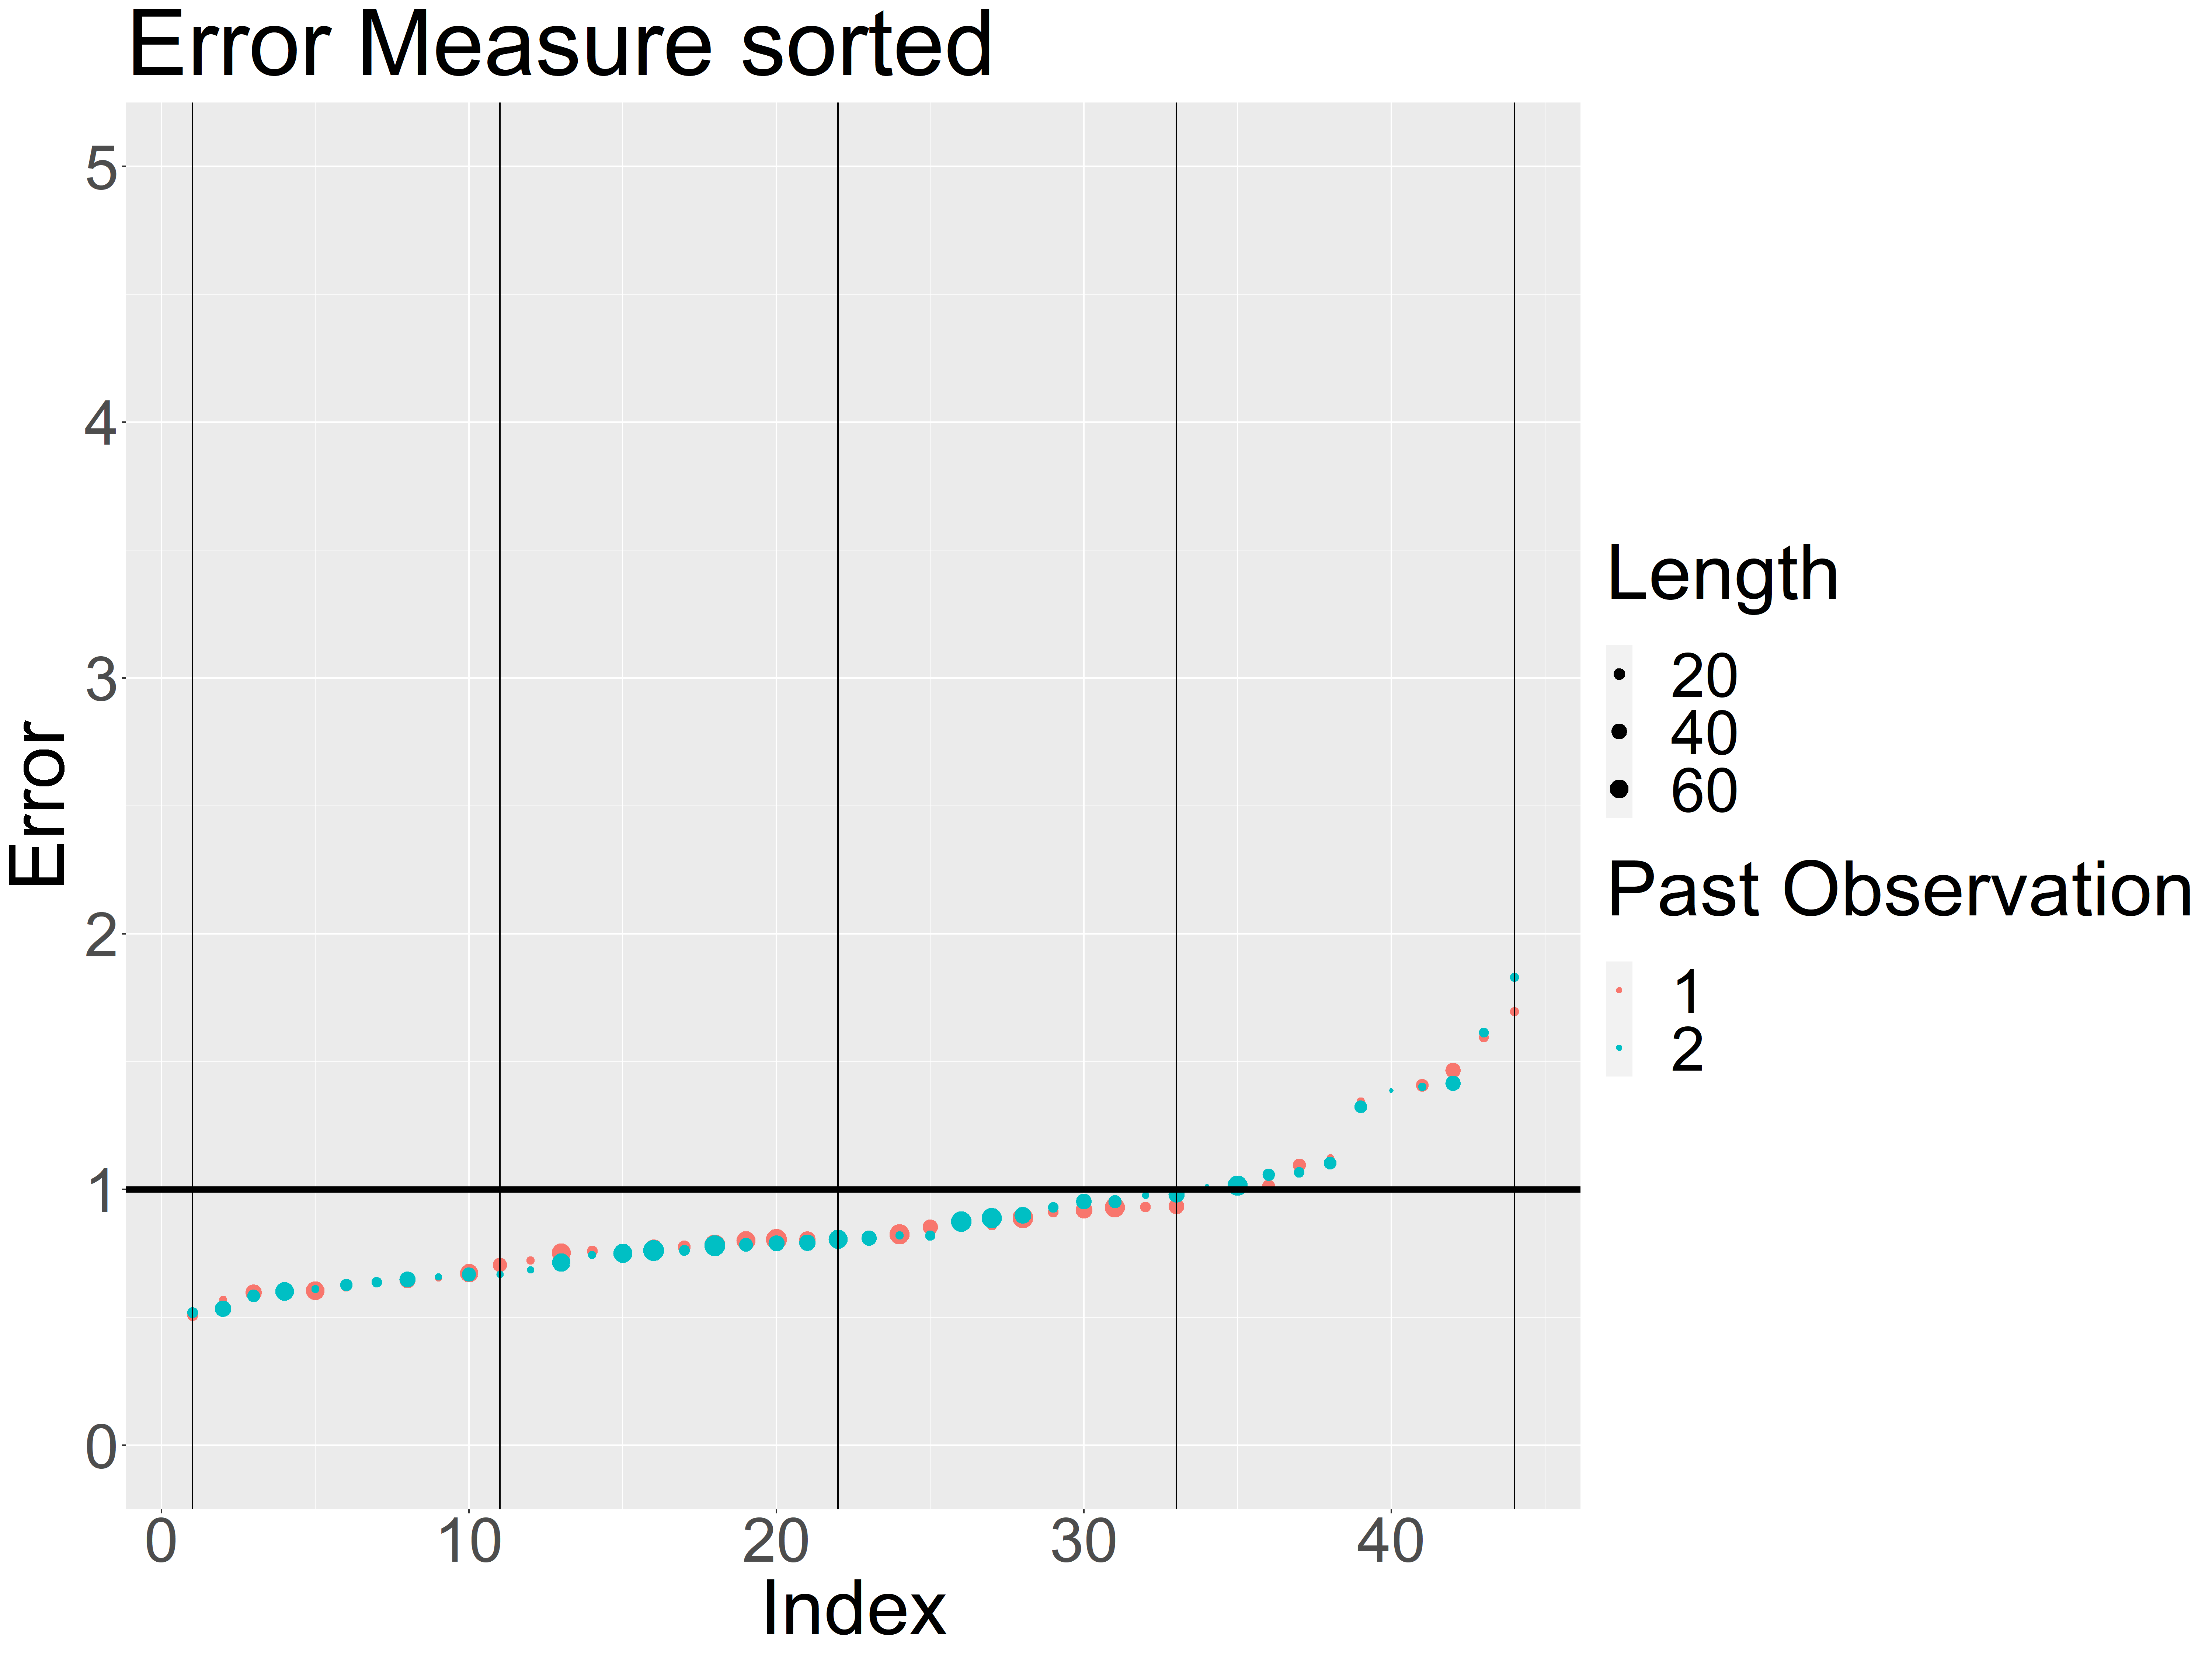
\includegraphics[width=\textwidth]{ErrorMeasureINGARCH_Quant_all__Variation_pastOb.png}
\caption{Quantiles for a different number of past observations}
\label{fig:past obs Quant}
\end{subfigure}
\caption{Comparison of a different number of past observations}
\label{fig:past obs Comp1}
\end{figure}

